


\chapter{Reconstrucción}
\section{Introducción}
A la salida del bloque de detección de marcadores se tiene, para cada cámara y para cada cuadro de una secuencia adquirida, un conjunto de coordenadas en dos dimensiones $(x,y)$ que ubican la posición en la imagen de aquellos marcadores que fueron detectados.
El proceso de reconstrucción consiste en obtener las coordenadas en tres dimensiones de la posición de los marcadores en el espacio a partir de las coordenadas en dos dimensiones obtenidas en el bloque anterior.
En la figura \ref{fig: esquema_reconstruccion} se muestra un ejemplo de reconstrucción de un marcador usando para esto la detección de marcadores en dos cámaras.\\

\begin{figure}[!ht]
\begin{center}
%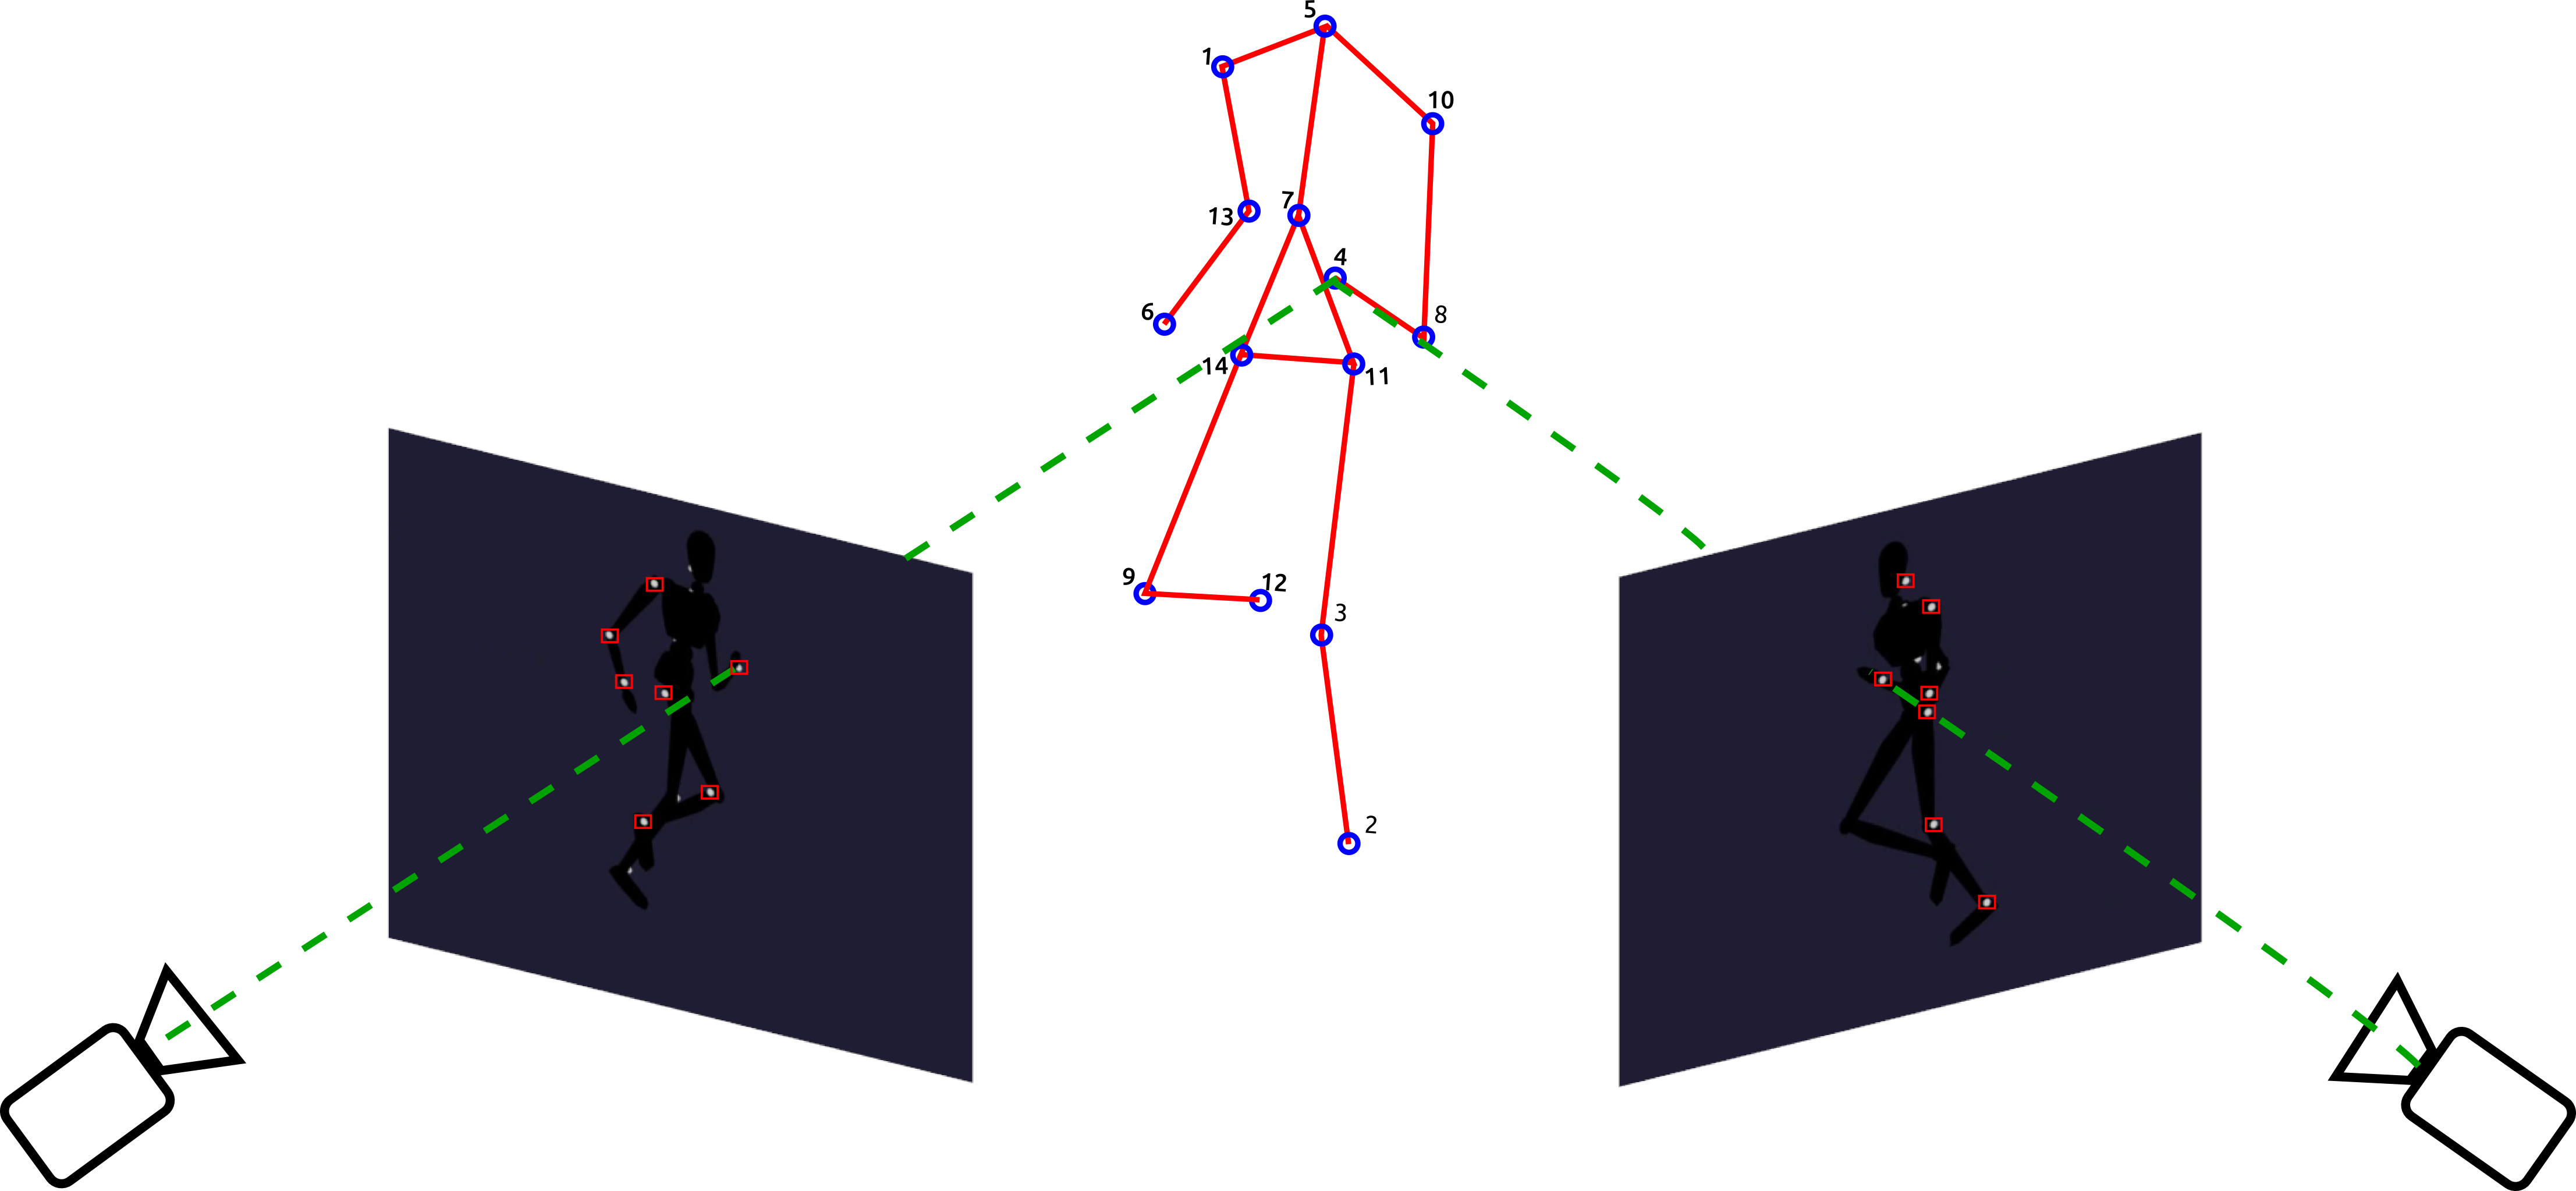
\includegraphics[scale=0.20]{img/Reconstruccion/ejemplo_reconstruccion.png}
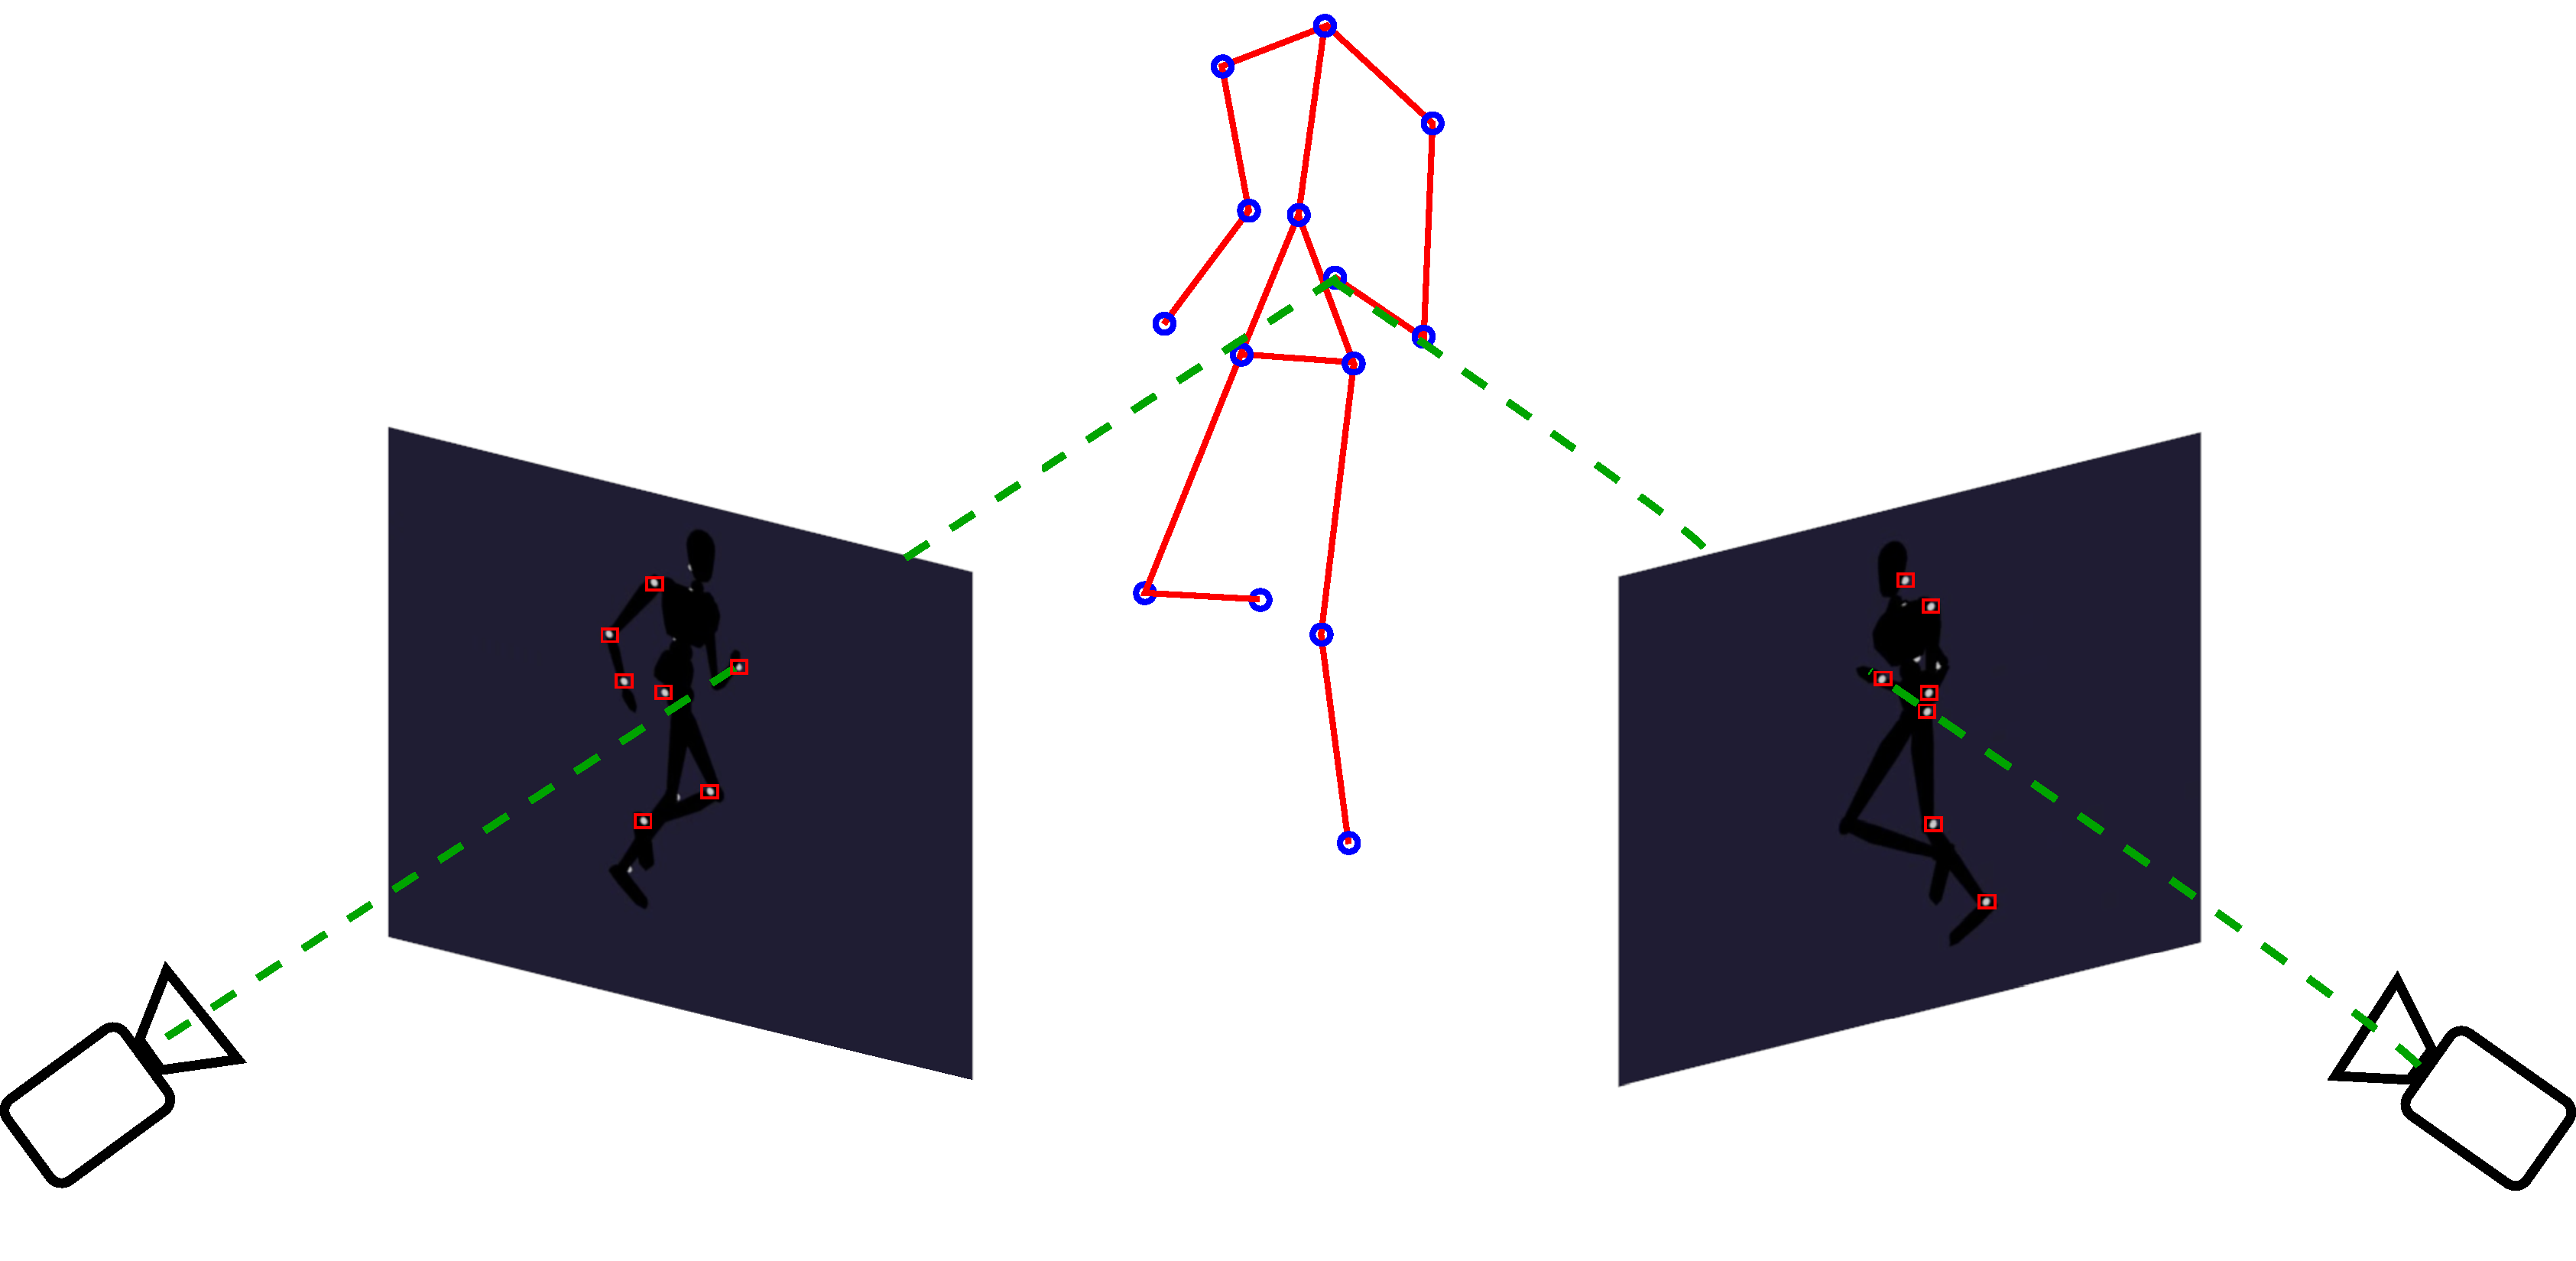
\includegraphics[scale=0.20]{img/Reconstruccion/reconstruccion}

\end{center}
\caption{Reconstrucción con dos cámaras}
\label{fig: esquema_reconstruccion}
\end{figure}

%Se observa en la figura a uno de los marcadores detectados desde las dos vistas y su correspondiente punto 3D reconstruido.\\
El proceso de reconstrucción implementado consiste en tres pasos fundamentales:
\begin{enumerate}
\item Determinar aquellos marcadores detectados en las distintas cámaras que corresponden a un mismo marcador en el espacio. De esta manera se establece una correspondencia entre los marcadores detectados en las distintas vistas. Dichas asociaciones se establecen de a pares de cámaras.
\item Una vez establecidas estas correspondencias se selecciona aquella que con algún criterio pueda considerarse con mayores posibilidades de ser una asociación correcta. Luego se determina la posición en el espacio del marcador a partir de la asociación seleccionada.
\item Una vez reconstruido uno de los marcadores debe verificarse si dicho marcador fue detectado en el resto de las cámaras.
\end{enumerate}
\begin{figure}[H]
\begin{center}
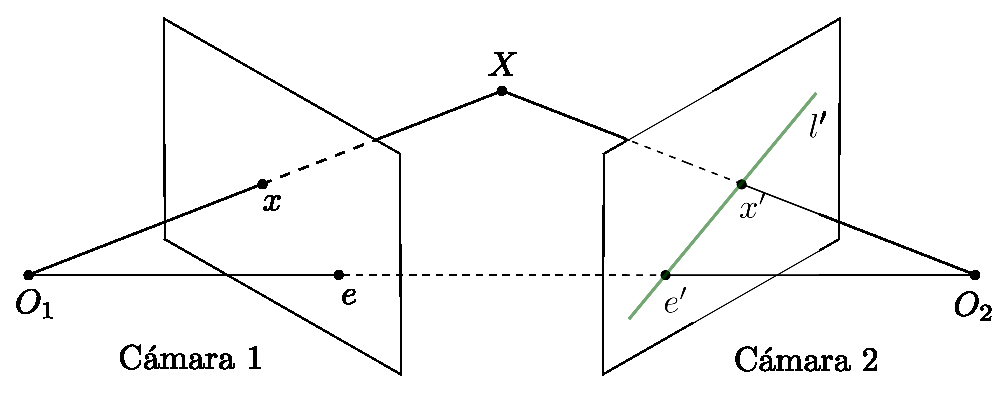
\includegraphics[scale=0.7]{img/Reconstruccion/geometria_epipolar}
\end{center}
\caption{Geometría epipolar}
\label{fig: geometria_epipolar}
\end{figure}

\section{Geometría epipolar}



Para explicar el algoritmo de reconstrucción es necesario describir brevemente algunos conceptos fundamentales de la geometría epipolar.  Dicha geometría es la que se presenta cuando dos cámaras en distintas posiciones se encuentran capturando el mismo espacio 3D. El análisis de esta situación permite obtener relaciones entre los puntos 3D con sus correspondientes proyecciones en las cámaras, así como las relaciones entre los propios puntos proyectados en las distintas cámaras\cite{cyganek}\cite{hartley}. \\

 Como se muestra en la figura \ref{fig: geometria_epipolar}, se tiene el caso en que dos cámaras observan un mismo punto 3D en el espacio, el punto $X$. Para esto se considera el modelo \textit{pinhole} de la cámara  descrito en la sección \ref{calibracion}. En ese caso los puntos $O_1$ y $O_2$ son los centros o focos de las cámaras.\\
 
  El punto $X$ se proyecta en dichas cámaras en los puntos $x$ y $x'$. Es decir, $x$ pertenece a la intersección de la retina de la cámara 1, con la recta $\overline{O_1X}$, análogamente el punto $x'$ pertenece a la intersección de la retina de la cámara 2 con la recta $\overline{O_2X}$. A su vez, los focos de ambas cámaras $O_1$ y $O_2$ definen una recta que corta a las retinas de las cámaras en los puntos $e$ y $e'$, llamados epipolos.\\
  
  Si el punto $X$ varía sobre el espacio 3D, se tienen múltiples rectas que pasan por dicho punto y el foco de la cámara 1, el punto $O_1$. Dado que $O_1$ se proyecta en la cámara 2 como el punto $e'$ en el plano imagen, todas las rectas  $\overline{O_1X}$ se proyectan en dicha cámara como rectas que se intersecan en el punto $e'$, a estas rectas se le denominan rectas epipolares. Análogamente las rectas 3D $\overline{O_2X}$ se proyectan sobre la cámara 1 como rectas epipolares que se intersecan en el punto $e$. De esta manera se tiene que los puntos $X$, $O_1$ y $O_2$ forman un plano, llamado plano epipolar,  que interseca a los planos imagen en las rectas epipolares.\\
  
De lo anterior se observa que si se conoce la proyección $x$ de un punto $X$ sobre una de la cámara 1, también se conoce la recta epipolar $\overline{e'x'}$ y el punto $X$ se proyecta en la cámara 2 en un punto $x'$ situado en dicha recta epipolar. Esto implica que por cada punto visto en una retina en la otra se observa como una línea.\\
 
Si los puntos $x$ y $x'$ son conocidos, sus proyecciones son también conocidas y si estos puntos corresponden a un mismo punto 3D su lineas de proyección deben interceptarse en $X$. Por lo tanto las coordenadas del punto X pueden derivarse a partir de las coordenadas de sus puntos imagen.\\
 
Para el caso de cámaras reales se tienen distorsiones de ruido, imperfecciones en las lentes de las cámaras, etc. que producen que las proyecciones sean tal que el punto 3D, su proyección en la cámara y el foco de la misma no sean colineales, por lo tanto la proyección real de un punto 3D va a ser aproximadamente el punto ideal de su proyección. \\

\subsection{Matriz Fundamental}

La matriz fundamental es la representación algebraica de la geometría epipolar. Si se tiene el punto $X$ y sus correspondientes proyecciones $x$ y $x'$ en las cámaras, se tiene que se verifica la siguiente condición :

\begin{equation}
(x')^T F x = 0
\label{ec: matriz fundamental}
\end{equation}
si  $F$ la matriz fundamental y $x$, $x'$ están en coordenadas homogéneas.\\

Si se tienen, de la cámara 1, la matriz de proyección $P$ y $x$, el punto $X$ se encuentra en la recta de proyección, que puede describirse en forma paramétrica:

\begin{equation}
	X(\lambda) = P^+x+\lambda O_1
\end{equation}

donde $P^+$ es la pseudo-inversa, tal que $PP^+=I$.\
En particular se toman dos puntos de esa recta, el punto $P^+x$ ($\lambda = 0$) y el punto $O_1$ ($\lambda = \infty$).\
Si se proyectan estos puntos en la cámara 2 se obtienen los puntos $P'P^+x$ y $P'O_1$ respectivamente, siendo $P'$ la matriz de proyección de la cámara 2. Estos puntos pertenecen a la recta epipolar:

\begin{equation}
l' = (P'O_1) \times (P'P^+ x)
\end{equation}

El punto $P'O_1$ es el epipolo $e'$ de la cámara 2. Por lo tanto $l' = e' \times (P'P^+) x$, entonces se define la matriz fundamental como:

\begin{equation}
F=e' \times P'P^+
\end{equation}

Si los puntos imagen se corresponden $x \leftrightarrow x'$, entonces $x'$ se encuentra en la recta epipolar $l'=Fx$ correspondiente al punto $x$, que implica que se cumpla $0=(x')^Tl'$ y por lo tanto se verifica la condición de la ecuación \ref{ec: matriz fundamental}. Como se explicó anteriormente esto se cumple en condiciones ideales pero no para cámaras reales en las que aparecen los efectos del ruido, etc. por lo tanto debe esperase que si se tiene un punto $x$ y su correspondiente $x'$, la ecuación \ref{ec: matriz fundamental} no verifique pero en cambio de un valor próximo a cero.\\

Algunas propiedades básicas de esta matriz son que si $F$ es la matriz fundamental del par de cámaras con matrices de proyección ($P,P'$), entonces $F^T$ es la matriz fundamental del par de cámaras en sentido opuesto: ($P',P$). Por otra parte si se tiene el punto $x$ en la imagen de una cámara, su recta epipolar correspondiente en otra cámara es $l'=Fx$. Análogamente $l=F^Tx'$ representa la línea epipolar a x' en la segunda cámara.

\section{Algoritmo propuesto por Herda }

Como se explicó anteriormente, se inicia la implementación de este bloque a partir del algoritmo propuesto por Herda \cite{herda}. Este algoritmo en algunos aspectos no es descripto con el detalle suficiente tal que pueda ser replicado fielmente. Por esta razón su implementación se ha realizado tomando algunas libertades en los casos en que su interpretación pueda ser algo ambigua.\\

Por otra parte este algoritmo plantea utilizar la información del esqueleto, como por ejemplo la posición de articulaciones, distancias entre marcadores, etc. Dado que este aspecto del algoritmo no fue implementado resultó necesario robustecer el proceso de reconstrucción en las partes del algoritmo donde no se utiliza esta información.\\


El algoritmo implementado por Herda utiliza la triangulación estéreo para reconstruir un punto 3D a partir de los puntos 2D detectados en las distintas vistas. La correspondencia entre distintas vistas se establece mediante la matriz fundamental, cuyos conceptos fueron explicados anteriormente. Esta matriz fundamental se obtiene mediante el proceso de calibración.\\

Los pasos que sigue el algoritmo se describen a continuación:\

\begin{itemize}
\item Se toman dos vistas y se realiza el test de la condición epipolar. Si existe una asociación no ambigua se reconstruyen  las coordenadas 3D a partir de las coordenadas 2D.

\item Las coordenadas 3D reconstruidas se re-proyectan en las cámaras restantes. Los puntos 2D encontrados en esa re-proyección son asociados al punto 3D. De esta forma se tiene por cada punto 3D , sus correspondientes puntos 2D asociados en las distintas vistas.\

\item Se considera que un marcador 3D está correctamente reconstruido si se re-proyecta en al menos una cámara. A este tipo de reconstrucción se le llama \textit{reconstrucción trinocular}.\\

\item Si el número de marcadores reconstruidos es inferior al número de marcadores que están colocados en la persona, entonces se realiza una segunda asociación entre dos vistas. En este caso la reconstrucción se realiza solamente con dos vistas \textit{reconstrucción binocular}.\\

\end{itemize}

Posteriormente el algoritmo plantea realizar ciertos chequeos sobre los puntos reconstruidos de manera de validarlos. Dichos chequeos utilizan información del esqueleto. Estos chequeos son de visibilidad y de oclusión.\\

Lo que se quiere verificar en dichos chequeos, es que para un determinado cuadro los marcadores sean efectivamente visibles por aquellas cámaras que los reconstruyeron y no están ocultos por alguna parte del cuerpo, lo que evidenciaría que las reconstrucción es incorrecta. Si esto se verifica el algoritmo busca otras vistas de las cuales reconstruir el marcador.\\

\section{Algoritmo implementado}

El algoritmo implementado recibe como entrada los puntos 2D de los marcadores detectados y devuelve como salida los puntos 3D reconstruidos. El primer paso consiste en establecer una asociación entre ciertos puntos 2D de distintas cámaras. Luego pasa a conjunto de bloques que se ejecutan de manera iterativa hasta que no quedan marcadores para reconstruir. En dicho bloque se busca la mejor asociación encontrada, bajo determinado criterio, luego se reconstruye un punto 3D y se realiza un proceso de validación de dicho punto. En la iteración siguiente se actualizan las asociaciones que habían sido establecidas previamente. Cuando no hay más marcadores para reconstruir se detiene el proceso iterativo y se devuelve aquellos marcadores que fueron reconstruidos en cada iteración. En la figura \ref{fig: diagrama algoritmo} se presenta un diagrama del algoritmo.\\

\begin{figure}[H]
\hspace{-1cm}
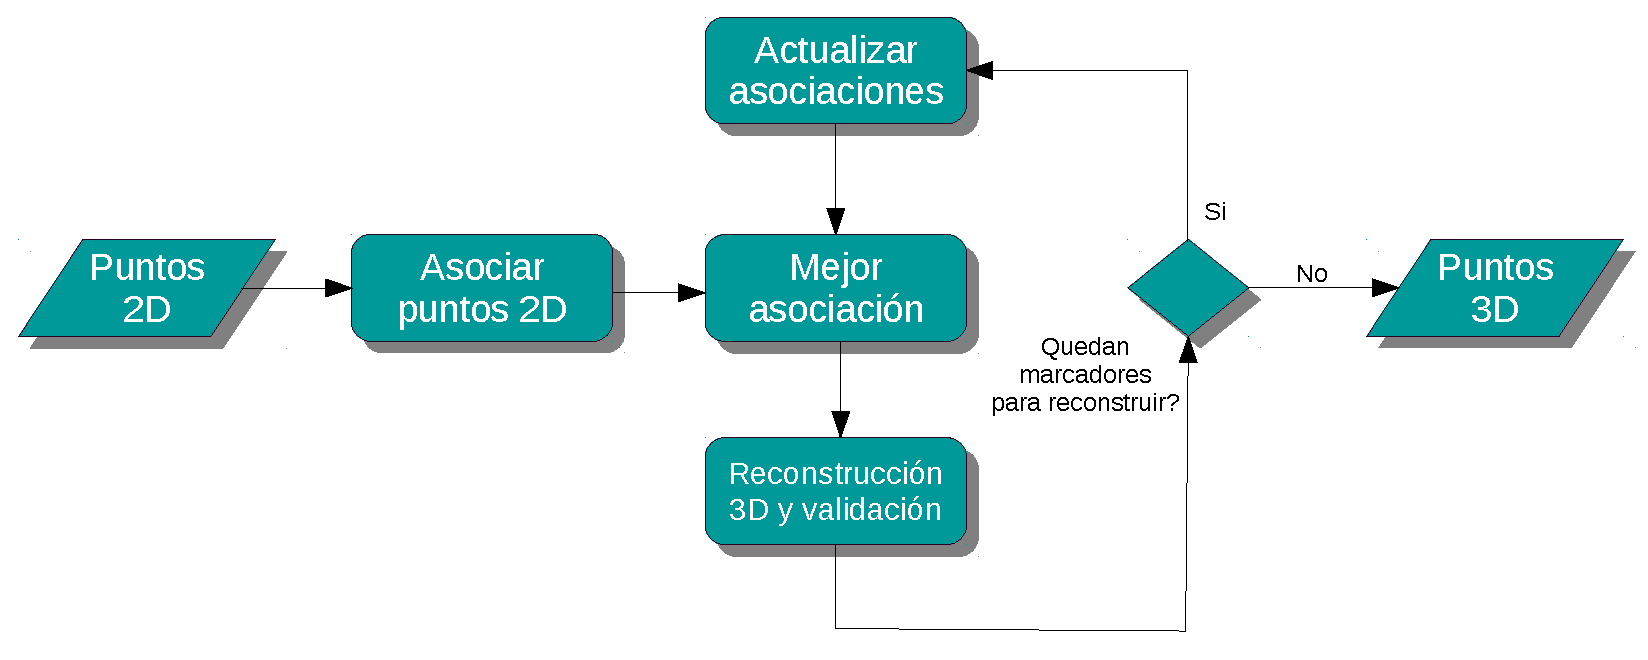
\includegraphics[scale=0.6]{img/Reconstruccion/diagrama_algoritmo.pdf}
\caption{Diagrama del algoritmo implementado}
\label{fig: diagrama algoritmo}
\end{figure}

A continuación se describe el funcionamiento de cada uno de los bloques:

\subsubsection{Asociar puntos 2D}

Este bloque recibe como entrada las coordenadas de los puntos detectados en cada una de las cámaras, parámetros de las mismas tales como sus matrices de proyección y devuelve para cada punto una lista ordenada por relevancia, de las asociaciones existentes con puntos en otras cámaras.
Basándose en lo explicado anteriormente el proceso  se puede ejemplificar  en la figura \ref{fig: cam2cam }. \\

\begin{figure}[H]
\begin{center}
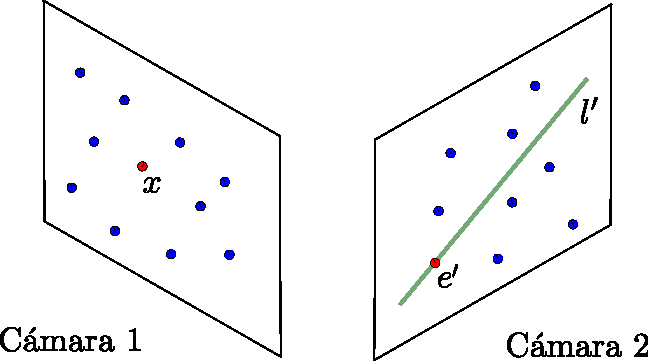
\includegraphics[scale=0.7]{img/Reconstruccion/cam2cam.pdf}
\end{center}
\caption{Asociación de puntos 2D en dos cámaras}
\label{fig: cam2cam }
\end{figure}

En primer lugar se seleccionan dos cámaras y se considera un punto en una de ellas, tomemos por ejemplo el punto $x$ de la cámara 1, y evaluemos la ecuación \ref{ec: matriz fundamental} para cada punto en la cámara 2. Esto equivale a proyectar la recta epipolar $l'$ correspondiente al punto $x$ sobre la cámara 2  y tomar las distancias de los puntos detectados en la cámara 2 a la recta $l'$. Se demuestra que dicha distancia difiere a menos de un factor de escala respecto al valor obtenido al evaluar la ecuación \ref{ec: matriz fundamental}. Se asume que los puntos de la cámara 2 que tengan mayor posibilidad de corresponder con el punto $x$, son aquellos que al ser evaluados por la ecuación obtienen valores próximos a cero.
De esta manera se obtiene para cada punto en la cámara 1 un conjunto de puntos en la cámara 2 ordenados según su distancia a la recta epipolar correspondiente.
Repitiendo el procedimiento de manera inversa, esto es, de la cámara 2 a la cámara 1, se obtiene igualmente para cada punto de la cámara 2  los puntos de la cámara 1 ordenados según su proximidad a la recta epipolar correspondiente. A continuación se toman otros pares de cámaras y se vuelve a iterar. 

Es importante resaltar que para la elección de los pares de cámaras se han considerado dos casos.
El primero de ellos evalúa cada cámara respecto a todas las restantes y el segundo considera la disposición de las cámaras en el espacio y empareja las cámaras adyacentes de manera consecutiva. Ver la figura \ref{img_asociacion}. %Más adelante se demuestra que este segundo procedimiento da mejores resultados.ACÁ SE DEBE REFERENCIAR BIEN DONDE ESTA ESA DEMOSTRACIÓN \\

 \begin{figure}[!ht]
   \centering 
    \subfloat[Cada cámara con las restantes]{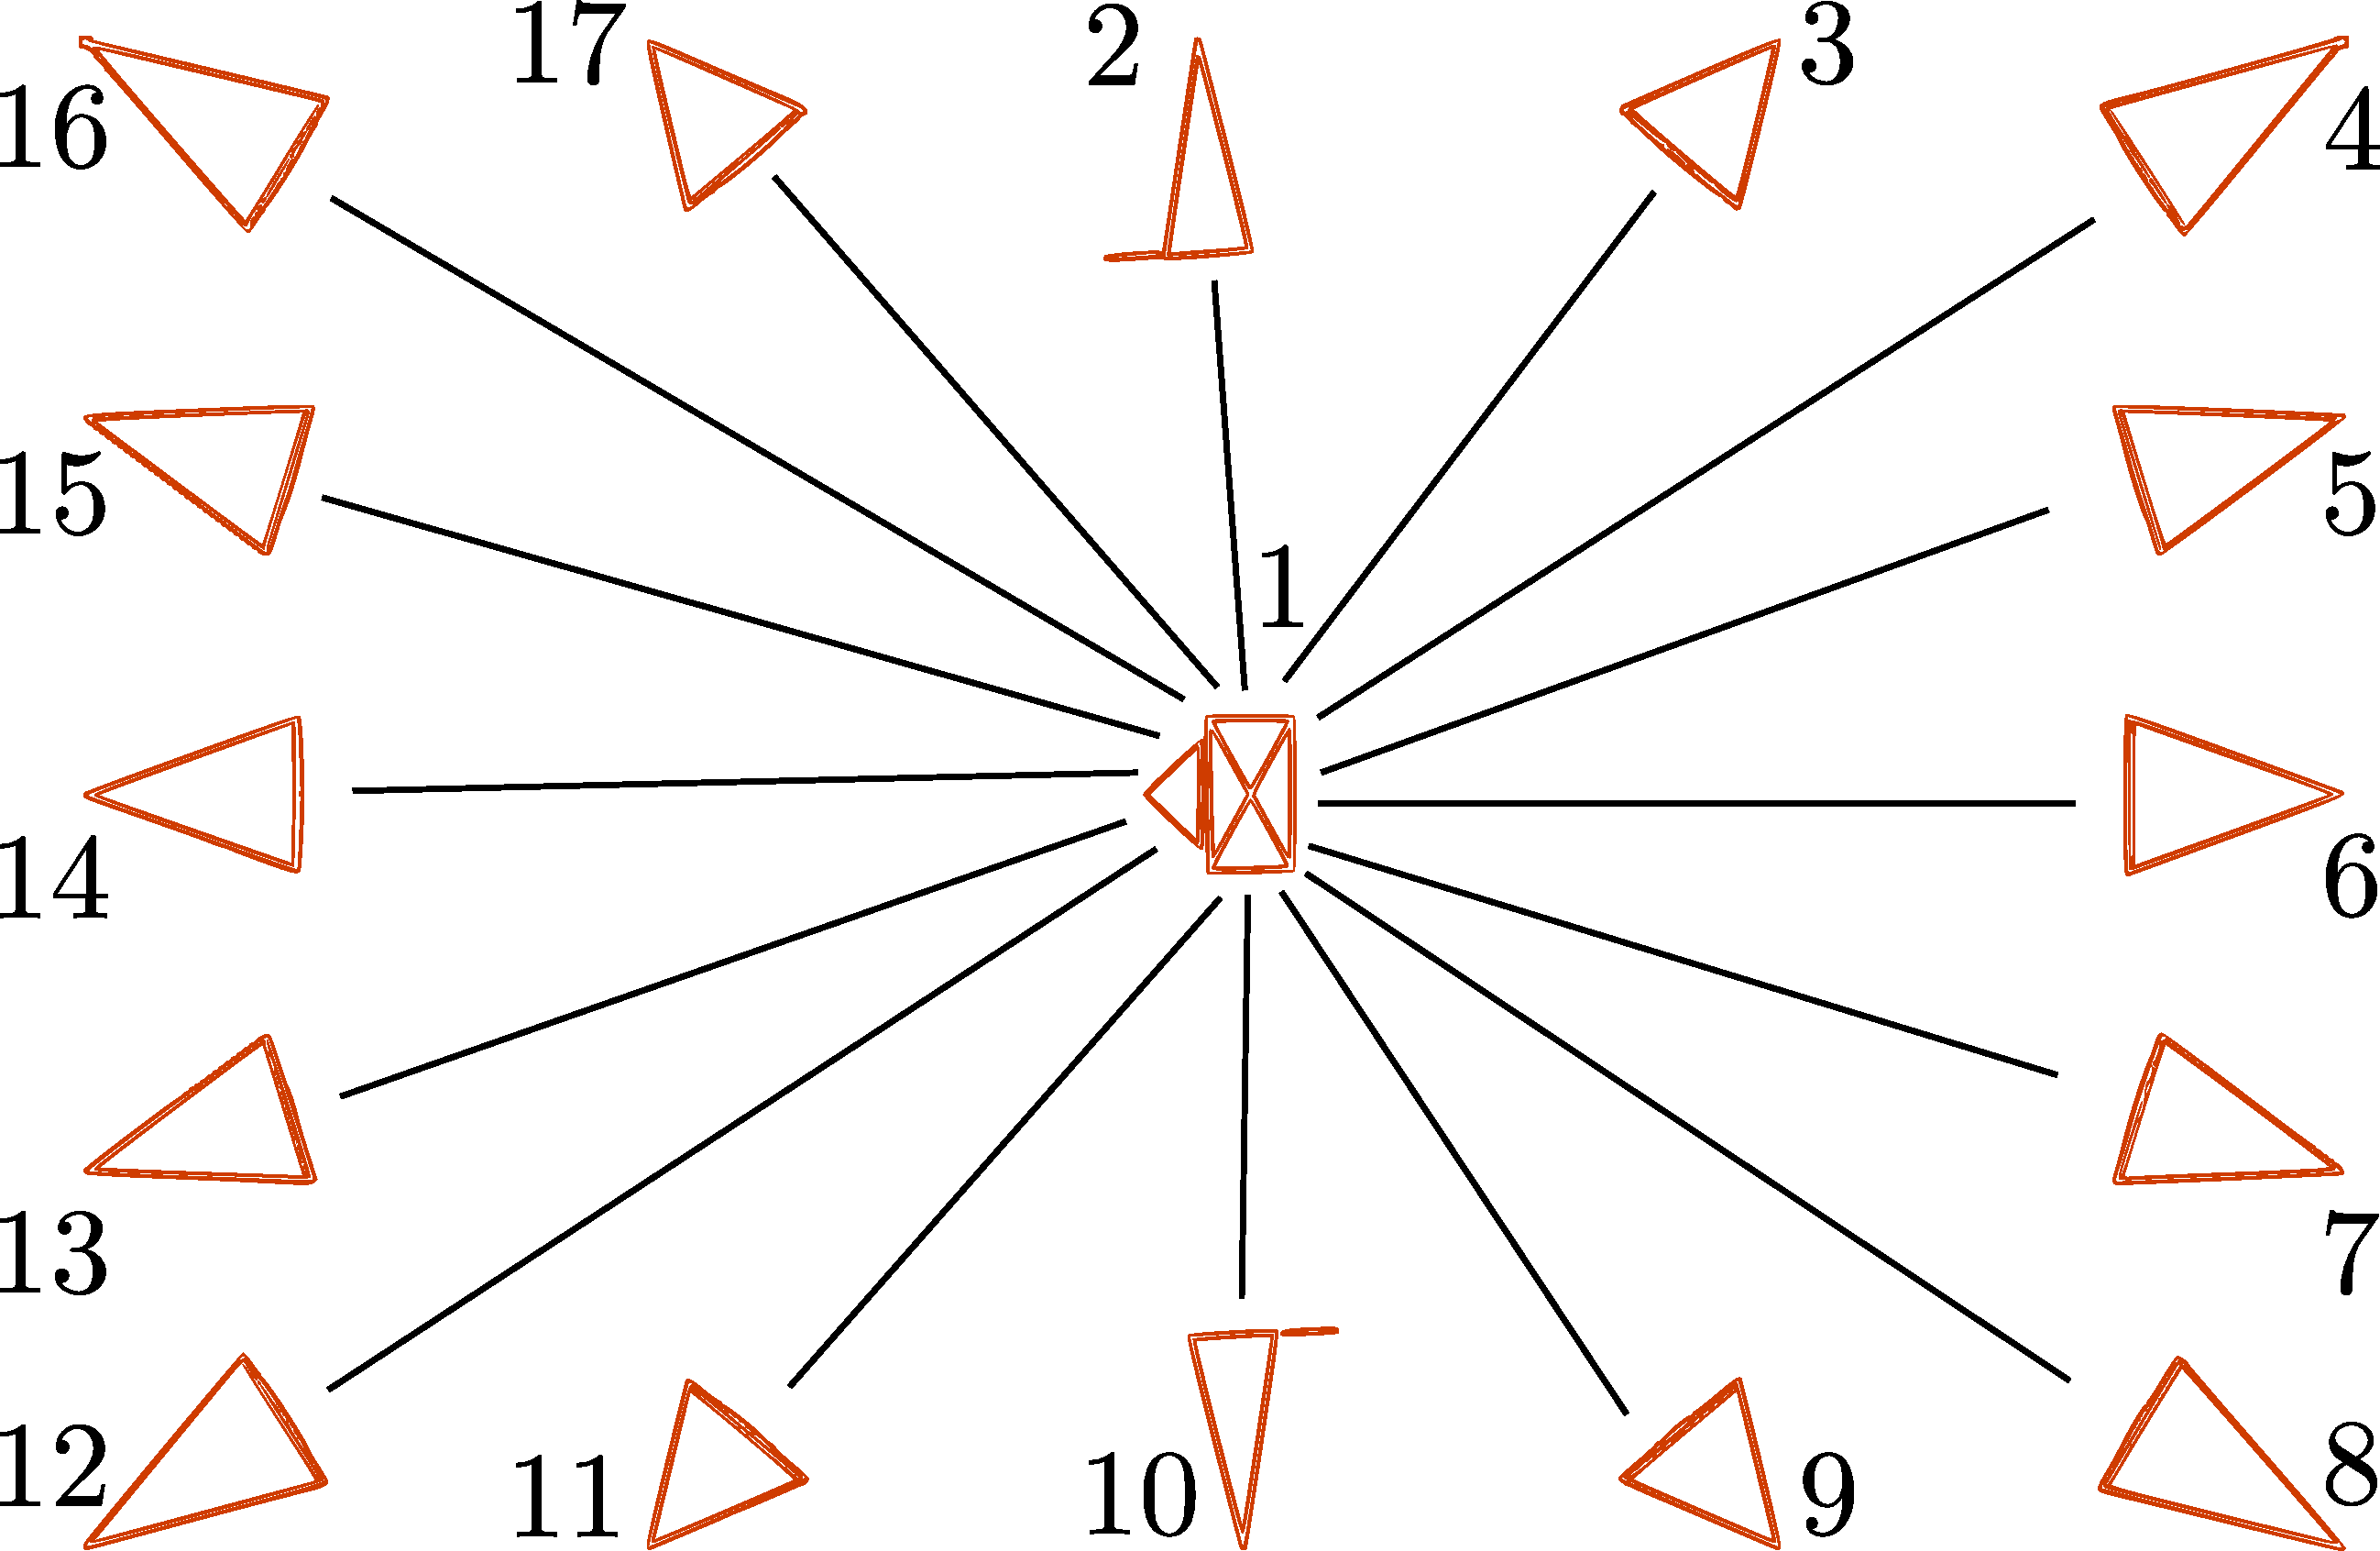
\includegraphics[scale=0.13]{img/Reconstruccion/enlazado_general}}\hspace{2cm}
    \subfloat[Cada cámara con su adyacente]{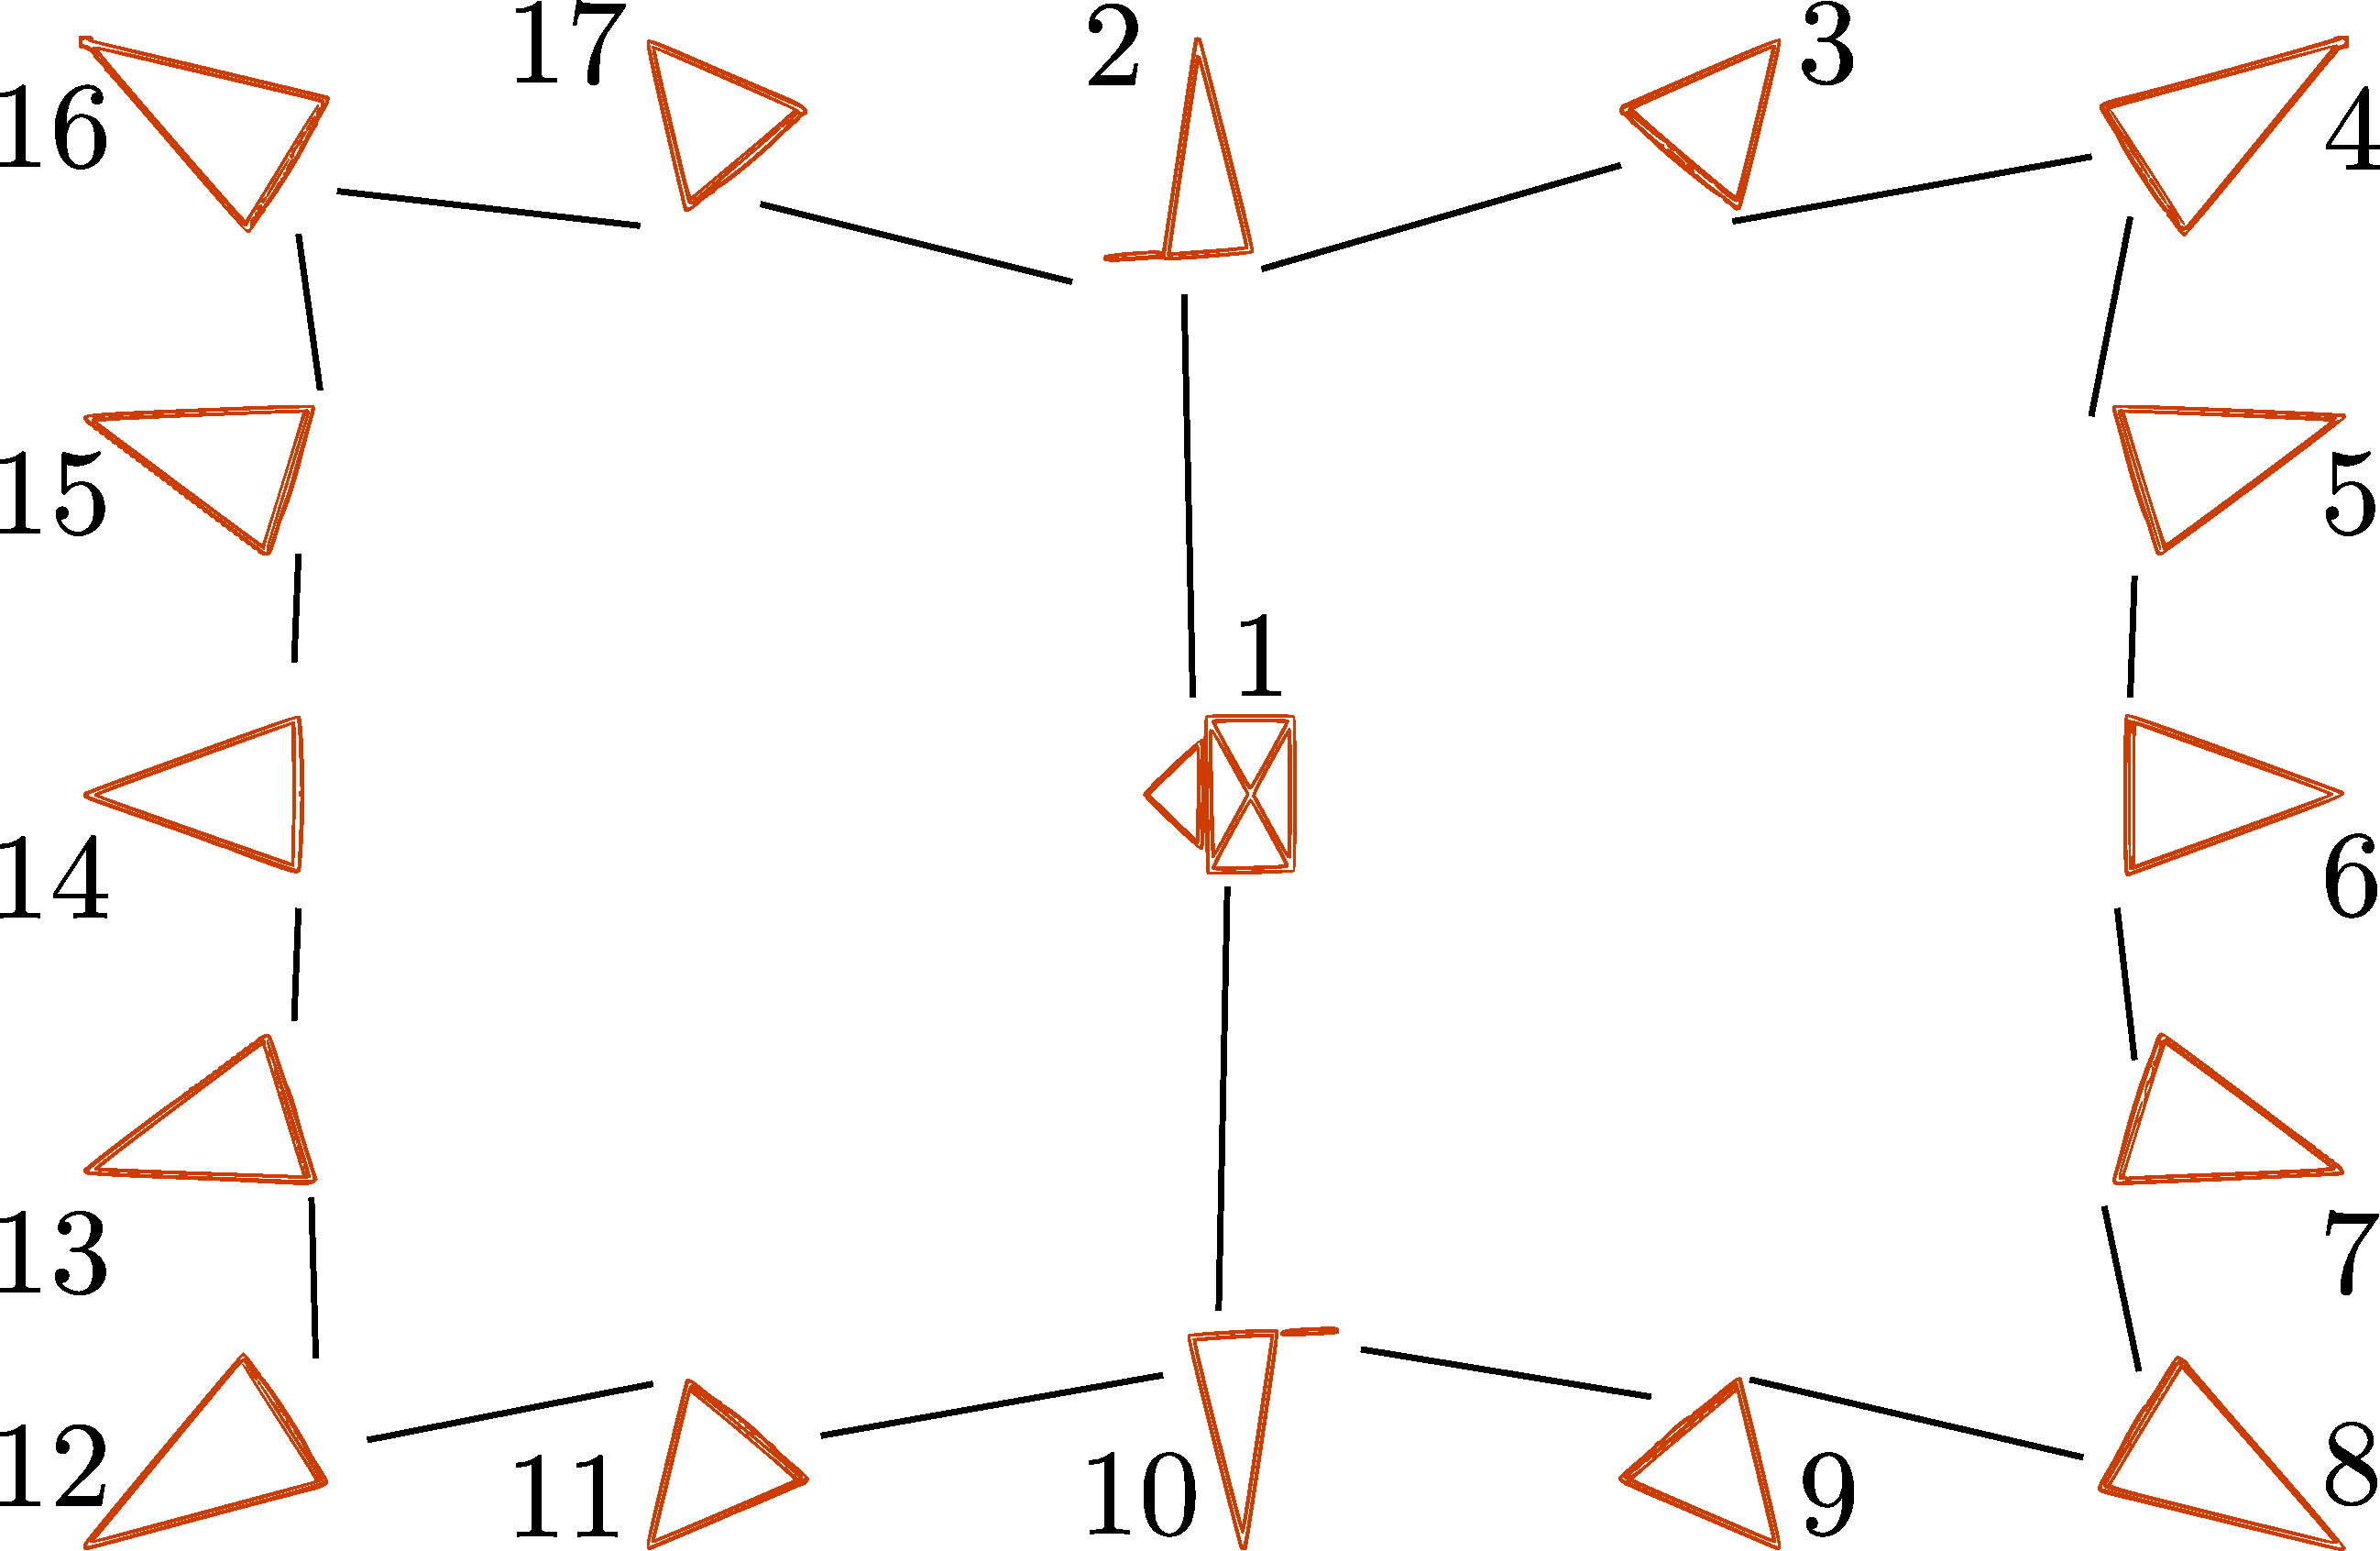
\includegraphics[scale=0.13]{img/Reconstruccion/enlazado_adyacente}\label{img_asociacion_consecutivas}}
   \caption{Métodos utilizados para generar pares de cámaras.}  
   \label{img_asociacion} 
 \end{figure} 





\subsection{Mejor asociación}

A partir de la lista con asociaciones entre puntos de dos vistas generada anteriormente, es necesario elegir aquella que posea mayor probabilidad de conformar la pareja de imágenes correspondiente a la proyección de un marcador 3D sobre dichas vistas.
%corresponder a la proyección en esas dos vistas de uno de los marcadores en el espacio.\\


Recordando que todas las asociaciones de puntos entre pares de cámaras se encuentran ordenadas por distancia, se toma aquella asociación que posea la menor distancia y contenga puntos válidos, descartando las restantes. Un punto se considera válido si en iteraciones anteriores no se a podido asociar a ningún punto 3D reconstruido, ver \ref{actualizar_asociaciones}.
De esta forma cada punto de una cámara es asociado, si existen puntos válidos, con un punto en otra de las cámaras.


 Supongamos en la figura \ref{fig: geometria_epipolar} que los puntos $x$ y $x'$ son la mejor asociación entre la cámara 1 y la cámara 2, y efectivamente son imágenes de un mismo punto 3D, idealmente los rayos de proyección se interceptarían en $X$, pero debido a incertidumbres en los procesos de calibración y segmentación la distancia entre dichos rayos no es nula, en el mejor de los casos solo es próxima a cero. 
Considerando esto último el procedimiento utilizado, para evaluar cual entre los pares de puntos asociados disponibles posee mayor posibilidad de corresponder a la proyección de un punto 3D, es proyectar todas los rayos de proyección y tomar aquella pareja de puntos que genere rayos de proyección con la menor distancia entre sí.


\subsection{Reconstrucción 3D y validación}\label{seccion_reconstruccion3D_validacion}


Luego de encontrar las mejores asociaciones entre dos cámaras se procede a reconstruirlas. Estas reconstrucciones deben ser validadas, para ello en principio se utiliza el  criterio propuesto por Herda \cite{herda}, se considera que una reconstrucción proveniente de dos cámaras es válida, si al proyectar sobre una tercer cámara existe al menos un punto de esta última que diste menos de un cierto valor umbral. Si efectivamente se encuentra al menos un punto, se asocia con los dos puntos que generaron la reconstrucción y se repite el proceso con el resto de las cámaras. Una vez finalizada la iteración, se retira a la pareja que genera la reconstrucción así como también a los puntos que lograron validarla, y se itera nuevamente repitiendo el proceso con la siguiente mejor pareja asociada entre dos cámaras.  


El algoritmo desarrollado si bien conceptualmente es similar, se implementa desde una óptica diferente computacionalmente más eficiente.
En lugar de llevar en cada iteración la información 3D a cada cámara, se procede a llevar la información de las cámaras una sola vez al espacio 3D y trabajar en cada iteración sobre el mismo. La información que contiene un punto en una retina se mapea en el espacio 3D sobre el rayo de proyección que contiene a dicho punto y al centro de la cámara correspondiente. Supongamos que tenemos los rayos de proyección en el espacio 3D de todos los puntos contenidos en las retinas, sea $x_1$ un punto en la cámara 1 de centro $O_1$ y $x_2$ punto en la cámara 2 de centro $O_2$, como se muestra en la figura \ref{img_reconstruccion_validacion}, consideremos que $x_1$ y $x_2$ se encuentran asociados y reconstruyen al punto $X_{12}$. Idealmente $X_{12}$ se genera al interceptar los rayos de proyección de los puntos $x_1$ y $x_2$, pero debido a incertidumbres en la detección de marcadores o la calibración, comúnmente los rayos se van a cruzar. La reconstrucción, se estima como el punto del espacio de menor distancia a ambos rayos, por lo que
$X_{12}$ se encuentra en el punto medio del segmento perpendicular a ambos rayos.


\begin{figure}[h!]
\centering
\hspace{-1cm}
\captionsetup{justification=centering,margin=1.0cm}
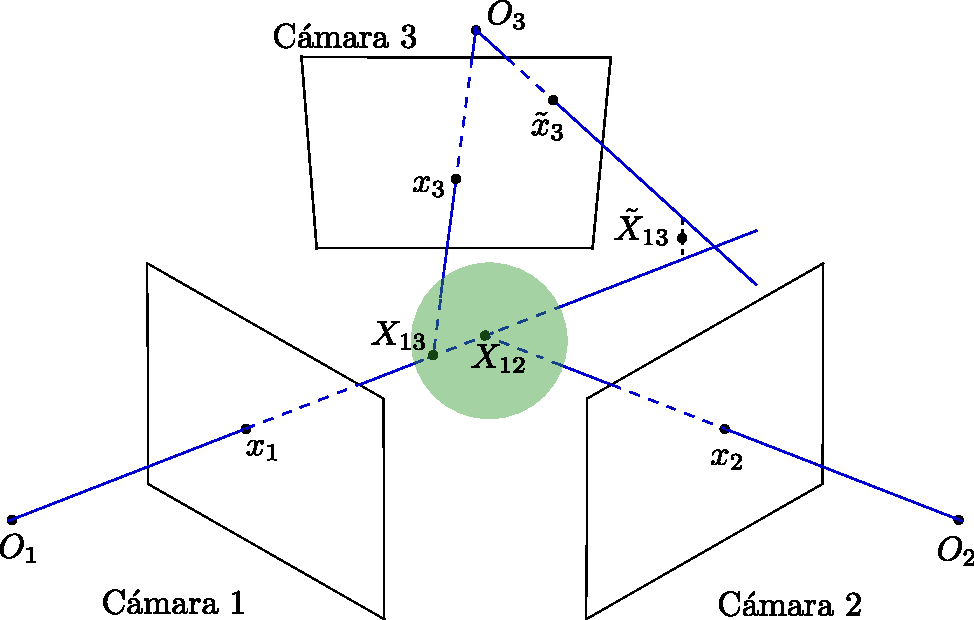
\includegraphics[scale=0.65]{img/Reconstruccion/validacion.pdf}
\caption{Reconstrucción entre cámaras 1, 2 y validación con cámara 3. El punto $x_3$ de la cámara 3 valida la reconstrucción, no así el punto $\tilde{x}_3$.}
\label{img_reconstruccion_validacion}
\end{figure}

El algoritmo implementado asume que un punto en una cámara valida a $X_{12}$ si junto a $x_1$ reconstruye un punto 3D que se encuentra dentro de la esfera $B(X_{12}, \delta)$ de centro $X_{12}$ y radio $\delta$, donde $\delta$ es un cierto valor umbral. Notar que la elección anterior de $x_1$ sobre $x_2$ es indiferente para nuestros propósitos. Si bien este criterio difiere del postulado original, en cierta manera se considera más robusto, pues en el postulado original basta con que dos puntos en una retina se encuentren lo suficientemente cerca para obtener una validación, pero esto no implica necesariamente que provengan de puntos 3D cercanos, sin embargo bajo el nuevo criterio si dos puntos 3D se encuentran cerca, entonces es válido afirmar que sus proyecciones sobre las distintas retinas también deben estarlo. Otra ventaja es que los umbrales bajo los cuales se considera que dos puntos están ``cerca'' difieren en cada una de las cámaras debido al distinto mapeo de distancias, sin embargo en el espacio 3D manejar un único umbral resulta suficiente.       

\subsection{Actualizar asociaciones}\label{actualizar_asociaciones}

Del bloque anterior se tiene, un punto $X$ reconstruido y sus correspondientes proyecciones en cada una de las cámaras. Dichas proyecciones no deben ser consideradas en próximas iteraciones, por tanto estos puntos 2D no se consideran puntos válidos.\\



Finalmente el proceso iterativo se detiene cuando no hay más marcadores para reconstruir, lo que implica que se cumplan cualquiera de las siguientes condiciones:\\
\begin{itemize}
\item el número de marcadores reconstruidos es igual al número de marcadores que tiene colocada la persona, o igual al número máximo de marcadores  reconstruidos que se haya indicado.

\item No existen puntos 2D válidos tal que pueda establecerse una asociación entre puntos de distintas vistas.
\end{itemize}




\section{Resultados de reconstrucción sobre secuencias sintéticas}

Se ha probado el algoritmo descrito anteriormente con secuencias capturadas en Blender. Para la configuración de 17 cámaras se han obtenido resultados aceptables,  con errores promedio menores a $0.5\,cm$. En la sección \ref{seccion_performance}, se define la medida de error  y se evalúa el desempeño del algoritmo respecto a dicha medida. En dichas pruebas se observan resultados aceptables aún utilizando 6 cámaras.

\begin{figure}[h!]
\centering
\captionsetup{justification=centering,margin=0.8cm}
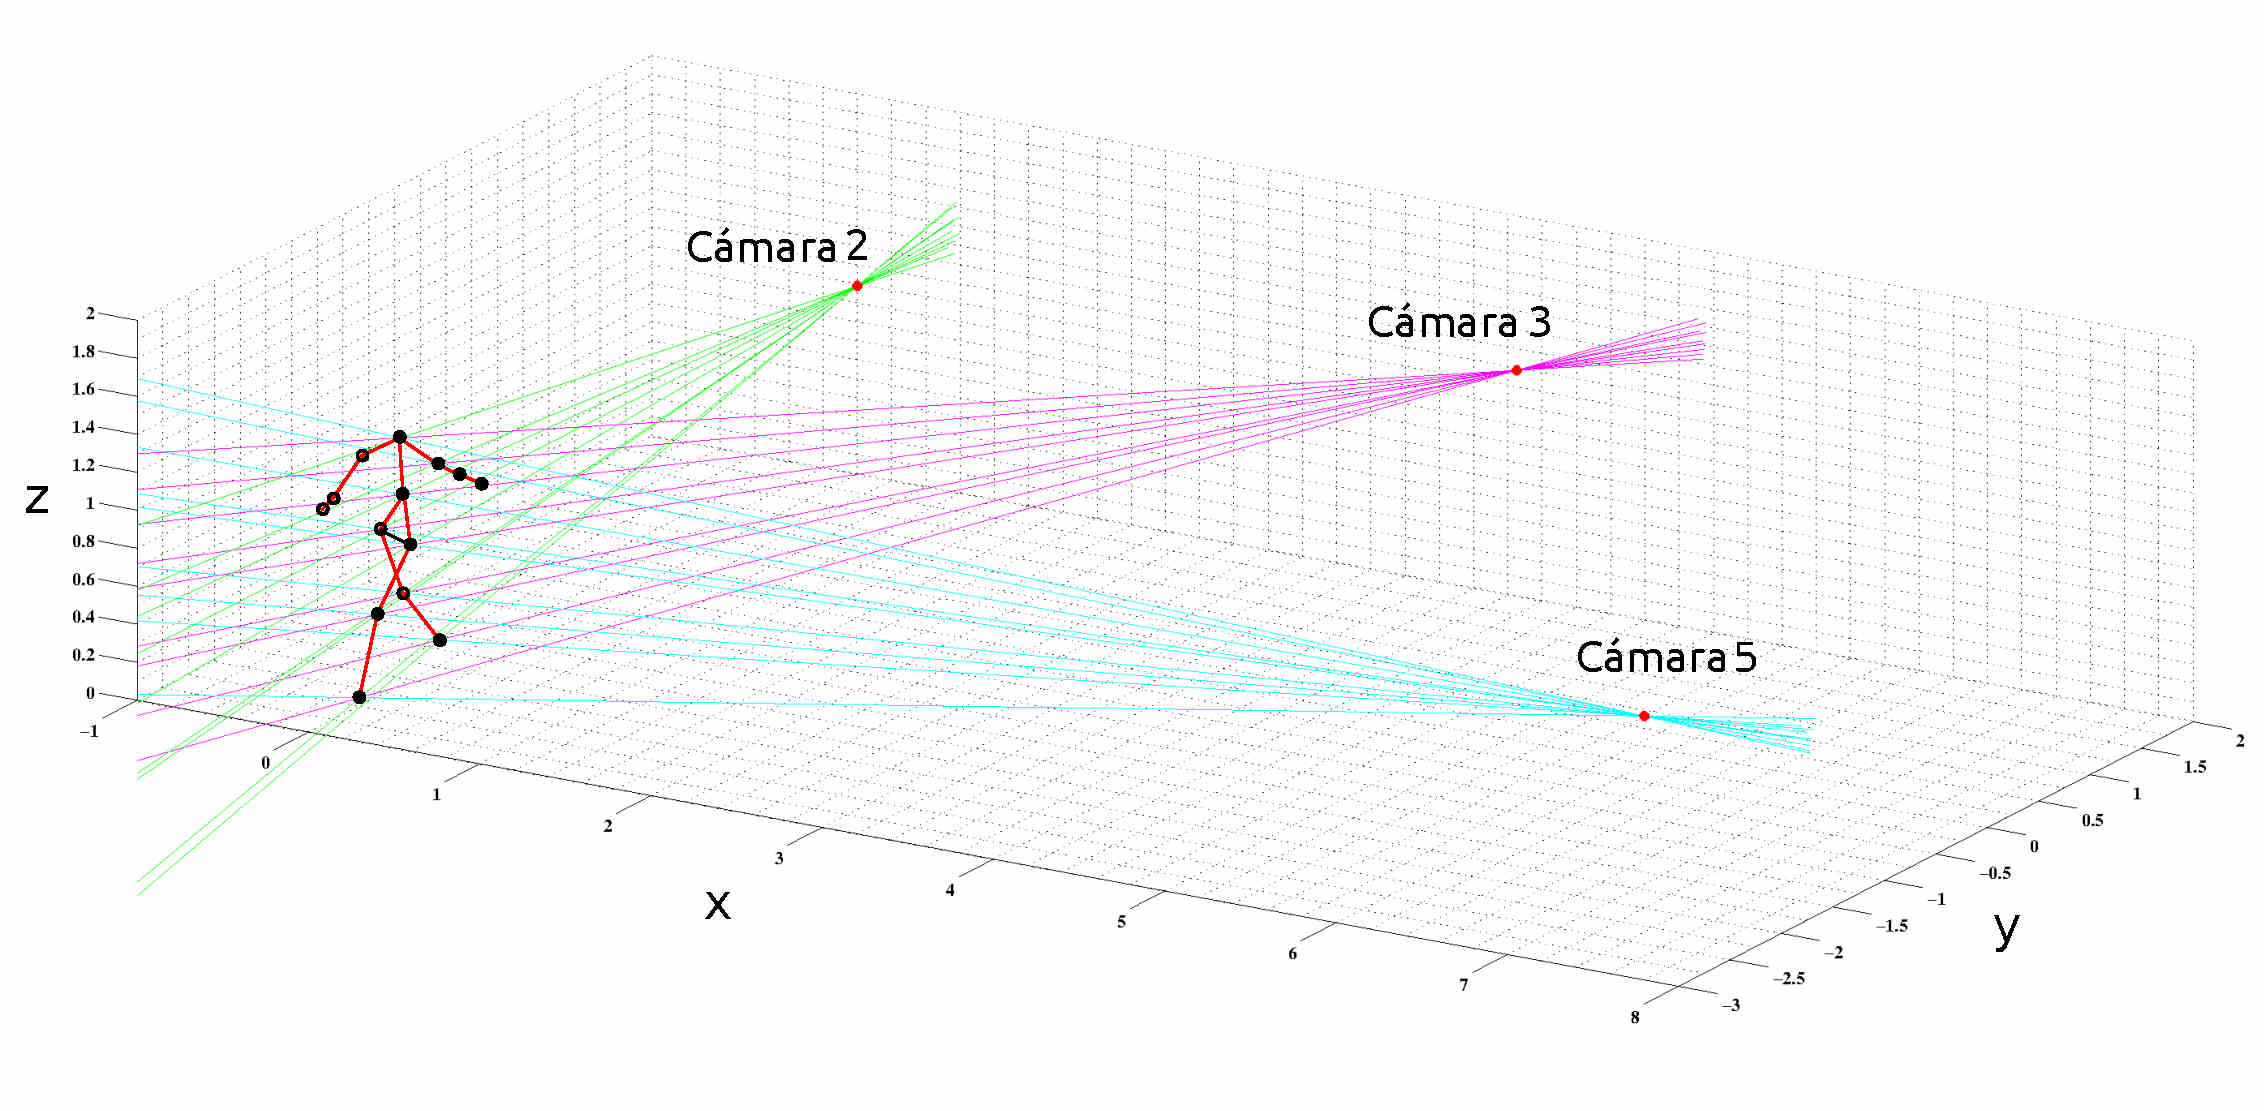
\includegraphics[scale=0.5]{img/Reconstruccion/Reconstruccion_3_camaras2.jpg}
\caption{Proceso de reconstrucción, ejemplo. Lo marcadores totalmente negros son los que se pudieron reconstruir utilizando información de las cámaras 2, 3 y 5.}
\end{figure}


Como se mencionó previamente se han realizado dos implementaciones distintas del bloque  “Asociar puntos 2D”. La primera de ellas considera las asociaciones de marcadores posibles entre pares de cámaras, evaluando cada una de las cámaras respecto a todas las restantes.  La segunda implementación toma en cuenta  la configuración circular de las cámaras en el espacio y se evalúa cada cámara con la que se encuentra inmediatamente más cerca,  recorriendo las cámaras en algún sentido.

\begin{table}[h]
\hspace{-1cm}
\begin{tabular}{cc|c|c|c|c|}
\cline{3-6}
                                                                              &                                                       & \multicolumn{2}{l|}{\textbf{Primera implementación}}                                                                                             & \multicolumn{2}{l|}{\textbf{Segunda implementación}}                                                                                            \\ \hline
\multicolumn{1}{|l|}{\begin{tabular}[c]{@{}l@{}}\textbf{Marker}\\ \textbf{Ground}\end{tabular}} & \begin{tabular}[c]{@{}l@{}}\textbf{Name}\\ \textbf{Ground}\end{tabular} & \begin{tabular}[c]{@{}l@{}}\textbf{Error} \\ \textbf{Promedio}\\ \textbf{(cm)}\end{tabular} & \begin{tabular}[c]{@{}l@{}}\textbf{Percentil}\\ \textbf{99\% (cm)}\end{tabular} & \begin{tabular}[c]{@{}l@{}}\textbf{Error}\\ \textbf{Promedio}\\ \textbf{(cm)}\end{tabular} & \begin{tabular}[c]{@{}l@{}}\textbf{Percentil}\\ \textbf{99\% (cm)}\end{tabular} \\ \hline
\multicolumn{1}{|l|}{1}                                                       & LeftUpLeg                                             & 0.4182                                                           & 3.7197                                                        & 0.3671                                                          & 0.5158                                                        \\ \hline
\multicolumn{1}{|l|}{2}                                                       & LeftLeg                                               & 0.3586                                                           & 0.5449                                                        & 0.3670                                                          & 0.5411                                                        \\ \hline
\multicolumn{1}{|l|}{3}                                                       & LeftFoot                                              & 0.3862                                                           & 1.0379                                                        & 0.3720                                                          & 0.5580                                                        \\ \hline
\multicolumn{1}{|l|}{4}                                                       & RightUpLeg                                            & 0.3963                                                           & 1.7542                                                        & 0.3714                                                          & 0.5879                                                        \\ \hline
\multicolumn{1}{|l|}{5}                                                       & RightLeg                                              & 0.3830                                                           & 0.9840                                                        & 0.3780                                                          & 0.5860                                                        \\ \hline
\multicolumn{1}{|l|}{6}                                                       & RightFoot                                             & 0.4192                                                           & 1.5364                                                        & 0.4212                                                          & 1.8483                                                        \\ \hline
\multicolumn{1}{|l|}{7}                                                       & Spine                                                 & 0.4075                                                           & 0.9092                                                        & 0.4040                                                          & 0.6043                                                        \\ \hline
\multicolumn{1}{|l|}{8}                                                       & Head                                                  & 0.4130                                                           & 1.2853                                                        & 0.3867                                                          & 0.9063                                                        \\ \hline
\multicolumn{1}{|l|}{9}                                                       & LeftArm                                               & 0.3626                                                           & 0.6394                                                        & 0.3666                                                          & 0.7997                                                        \\ \hline
\multicolumn{1}{|l|}{10}                                                      & LeftForeArm                                           & 0.4774                                                           & 2.8511                                                        & 0.3873                                                          & 0.9056                                                        \\ \hline
\multicolumn{1}{|l|}{11}                                                      & LeftHand                                              & 0.4217                                                           & 2.0700                                                        & 0.4007                                                          & 1.1722                                                        \\ \hline
\multicolumn{1}{|l|}{12}                                                      & RightArm                                              & 0.4756                                                           & 2.4363                                                        & 0.4025                                                          & 1.4771                                                        \\ \hline
\multicolumn{1}{|l|}{13}                                                      & RightForeArm                                          & 0.4590                                                           & 3.1711                                                        & 0.3844                                                          & 0.7810                                                        \\ \hline
\multicolumn{1}{|l|}{14}                                                      & RightHand                                             & 0.4545                                                           & 2.4782                                                        & 0.3816                                                          & 0.7728                                                        \\ \hline
\multicolumn{1}{l|}{}                                                         & \textbf{Secuencia }                                            & \textbf{0.38556 }                                                         & \textbf{1.7907    }                                                    & \textbf{0.35686}                                                         &\textbf{ 0.81266}                                                       \\ \cline{2-6} 
\end{tabular}
\caption{Performance de los algoritmos implementados en reconstrucción. }
\label{table_performance_reconstruccion}
\end{table}

En la tabla \ref{table_performance_reconstruccion} se muestra una comparación de resultados. En la misma se observa que en el segundo algoritmo implementado el error promedio mejora ligeramente respecto al primer algoritmo. Se observa también el error considerando el 99\% de los marcadores donde la mejora del segundo algoritmo es más significativa. Por esta razón se ha elegido la segunda de las implementaciones.
Una de las razones por las cuales puede suceder esto es que en el primer algoritmo se realizan búsquedas de asociaciones entre marcadores detectados, en pares de cámaras donde la probabilidad de que un mismo marcador sea visto por ambas cámaras puede ser muy baja. El ejemplo más representativo es cuando se consideran cámaras que están  ubicadas en posiciones diametralmente opuestas. En este caso las asociaciones que se encuentren tienen mayores posibilidades de ser asociaciones incorrectas, influyendo negativamente sobre el desempeño global del algoritmo. 



\section{Resultados de reconstrucción sobre secuencias reales}

Para probar la reconstrucción con secuencias reales se realizó la calibración según lo explicado en la sección \ref{seccion_calibracion_secuencias_reales}, por otra parte fue necesario robustecer el algoritmo de detección de marcadores como se explica en la sección \ref{resultadosyanalisissegmentacion}. Las pruebas del algoritmo presentado anteriormente realizadas sobre esta secuencia no han dado resultados aceptables, en este caso la mayoría de los marcadores se reconstruyen erróneamente. 


Con el fin de encontrar donde falla el sistema, se genera una secuencia sintética utilizando  para la captura tres cámaras en posiciones relativas que simula el caso real y se procede a probar el sistema con dichas secuencias.  En este caso los resultados tampoco han sido aceptables. Tras varias pruebas se llega  a la conclusión de que la deficiencia del sistema es que el algoritmo de reconstrucción no es lo suficientemente robusto para el caso en que se utilizan pocas cámaras.\\
% % % % % % % % % % % % % % % % % % % % % % % % % % % %
% % % % % %Poner UNA FIGURA DEL RESULTADO MOSTRANDO QUE TAN MALO ES.
% % % % % % % % % % % % % % % % % % % % % % % % % % % % %
Esta situación ha motivado el desarrollo de mejoras sobre el algoritmo de reconstrucción. Los cambios se realizan sobre la implementación disponible del sistema, intentando lograr un desempeño aceptable sin modificar la estructura global del sistema.

\section{Mejoras del algoritmo de reconstrucción}


Se hicieron pruebas sobre la base sintética, nuevamente simulando la situación del caso real, con el fin de aislar los errores provenientes de la calibración y de la detección de marcadores.
El algoritmo que se implementa en este caso tiene una estructura similar al considerado anteriormente, ver la figura \ref{fig: diagrama algoritmo}. Aunque algunos bloques modifican su funcionamiento, fundamentalmente el primero  “Asociar puntos 2D”.

\subsection{Asociar punto 2D}

En esta versión modificada el resultado de Asociar puntos 2D continúa siendo una lista ordenada de asociaciones entre puntos de distintas cámaras, pero el procedimiento para generar dicha lista es diferente.  Ahora dicho bloque se encarga  de comparar  las distancias de los rayos de proyección entre pares de cámaras, para encontrar parejas de puntos que presumiblemente sean imágenes de un mismo punto 3D.  

Asumiendo que las cámaras están colocadas alrededor del área de captura, el criterio utilizado para seleccionar los pares de cámaras a comparar es emparejar las cámaras adyacentes de manera consecutiva, como se muestra en la figura  \ref{img_asociacion_consecutivas}.

En cada par de cámaras seleccionado se consideran todos los rayos de proyección correspondientes a los puntos sobre ambas retinas. Con  cada punto de la primer cámara se genera una lista que contiene los puntos de la segunda cámara, ordenados según  la distancia euclídea existente entre los rayos de proyección asociados a los puntos de la cámara 2  con el rayo de proyección del punto de la cámara 1 considerado. 


Se repite el procedimiento hasta que sean comparadas todos los pares de cámaras consecutivas. De esta forma se obtiene una matriz de distancias entre rayos de proyección 3D para los diferentes pares de cámaras considerados.

\begin{figure}[h!]
\centering
\captionsetup{justification=centering,margin=2.8cm}
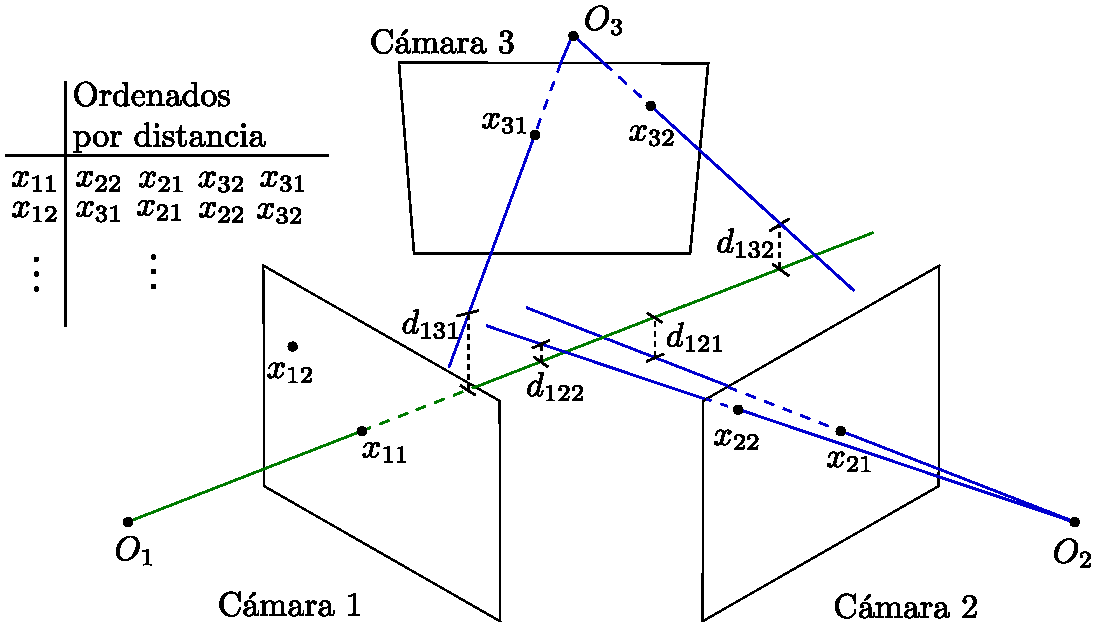
\includegraphics[scale=0.7]{img/Reconstruccion/Asociar_puntos_2}
\caption{Nueva asociación de puntos entre pares de cámaras.}
\end{figure}
 
\subsection{Mejor asociación}


Este bloque mantiene su funcionalidad, encontrar la pareja de puntos entre dos vistas, con mayor probabilidad de corresponder a la proyección de un punto 3D.
La diferencia fundamental con su implementación anterior es la gestión de las matrices de entrada, pues el ordenamiento por distancia de dichas matrices es diferente. En la primera implementación las distancias que producen el ordenamiento son generadas entre rectas epipolares y puntos, o sea distancias sobre un plano, mientras que en esta implementación las distancias son entre rayos en el espacio 3D.


Manteniendo el criterio original para implementar este bloque, el cual consiste en tomar la pareja de puntos que genere rayos de proyección con la menor distancia entre sí. 
La nueva entrada proporcionada por “Asociar puntos 2D” simplifica la nueva implementación.


Una vez que se tiene la matriz de distancias con todas las asociaciones de puntos entre los pares de cámaras considerados. Este bloque simplemente toma de entre todas las asociaciones disponibles de puntos válidos, aquel par de puntos que posea menor distancia asociada.
Recordar que un punto se considera válido si en iteraciones anteriores no se ha podido asociar a ningún punto 3D reconstruido.

\subsection{Resto de los bloques}

Los bloques de reconstrucción 3D y validación, y el de actualizar asociaciones realizan el mismo funcionamiento y tiene igual implementación que los utilizados en el algoritmo anterior. Ver las secciones \ref{seccion_reconstruccion3D_validacion} y \ref{actualizar_asociaciones}.

  Asimismo la condición que debe cumplirse para detener el proceso iterativo es la misma.
  
  
\section{Resultados del nuevo algoritmo}  
 
Se prueba el nuevo algoritmo para una secuencia sintética de 3 cámaras en las que se intenta simular el caso real. En este caso el sujeto cuenta con 14 marcadores. 
Los resultados muestran una mejora significativa respecto al algoritmo original
aunque no se llega a tener un desempeño ideal. 
De 20 cuadros relevados en 11 de ellos se logra reconstruir de manera aceptable los 14 marcadores, en 6 de los cuadros se tiene 1 marcador incorrectamente reconstruido y en los 3 restantes se tiene 2 marcadores incorrectamente reconstruidos.
En la figura \ref{img_reconstruccion_sintetica} se muestra el resultado de la reconstrucción para un cuadro  determinado de la secuencia sintética.\\

\begin{figure}[!ht]
   \centering 
    \subfloat[Vista derecha]{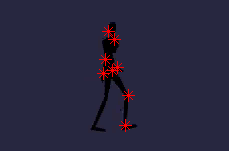
\includegraphics[scale=1.70]{img/Reconstruccion/50_derecha_sintetica.png}}\hspace{0.2cm}
    \subfloat[Vista  izquierda]{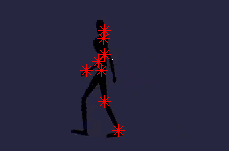
\includegraphics[scale=1.70]{img/Reconstruccion/50_izquierda_sintetica.png}}\hspace{2cm}
    \subfloat[Vista de atras]{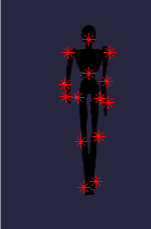
\includegraphics[scale=0.90]{img/Reconstruccion/50_atras_sintetica2.png}} \hspace{1.9cm}
    \subfloat[Resultado de la reconstrucción]{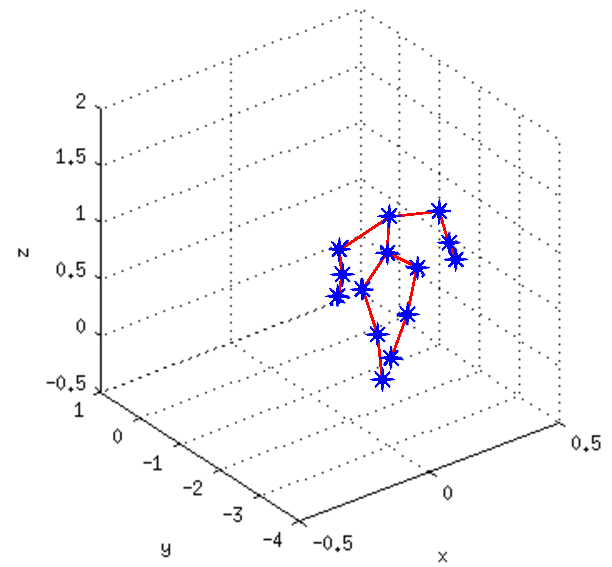
\includegraphics[scale=0.7]{img/Reconstruccion/50_matlab_sintetica.pdf}}    
   \caption{Reconstrucción de una secuencia sintética. Los asteriscos rojos indican los marcadores detectados.} 
   \label{img_reconstruccion_sintetica}    
\end{figure} 

Por último el nuevo algoritmo fue probado con secuencias reales. Si bien se reconstruyen varios marcadores mejorando la performance que se tenía con el algoritmo de reconstrucción inicial, los resultados no son tan alentadores como los obtenidos para las secuencias sintéticas. En cierta manera es esperable dado que en este caso se adicionan errores provenientes de las etapas de detección de marcadores y de calibración. En la figura \ref{img_reconstruccion_real2} se muestra el resultado obtenido para un cuadro de la secuencia real. 

\begin{figure}[!ht]
   \centering 
    \subfloat[Vista derecha]{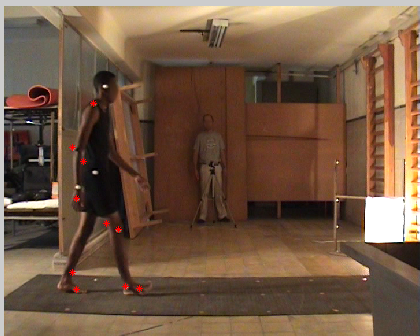
\includegraphics[scale=0.50]{img/Reconstruccion/22_derecha.png}}\hspace{0.8cm}
    \subfloat[Vista de atrás]{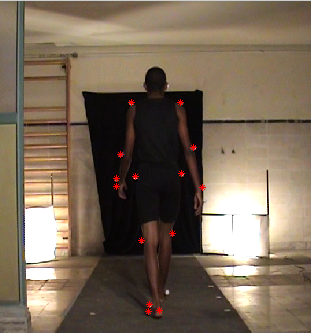
\includegraphics[scale=0.50]{img/Reconstruccion/22_atras.png}}\hspace{2cm}
    \subfloat[Vista izquierda]{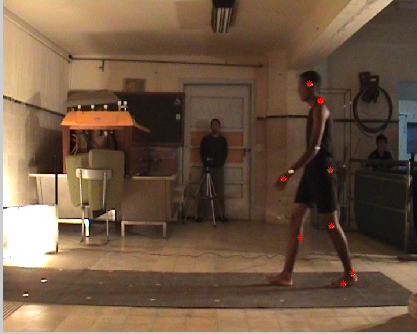
\includegraphics[scale=0.50]{img/Reconstruccion/22_izquierda.png}}\hspace{0.5cm}
    \subfloat[Resultado de la reconstrucción]{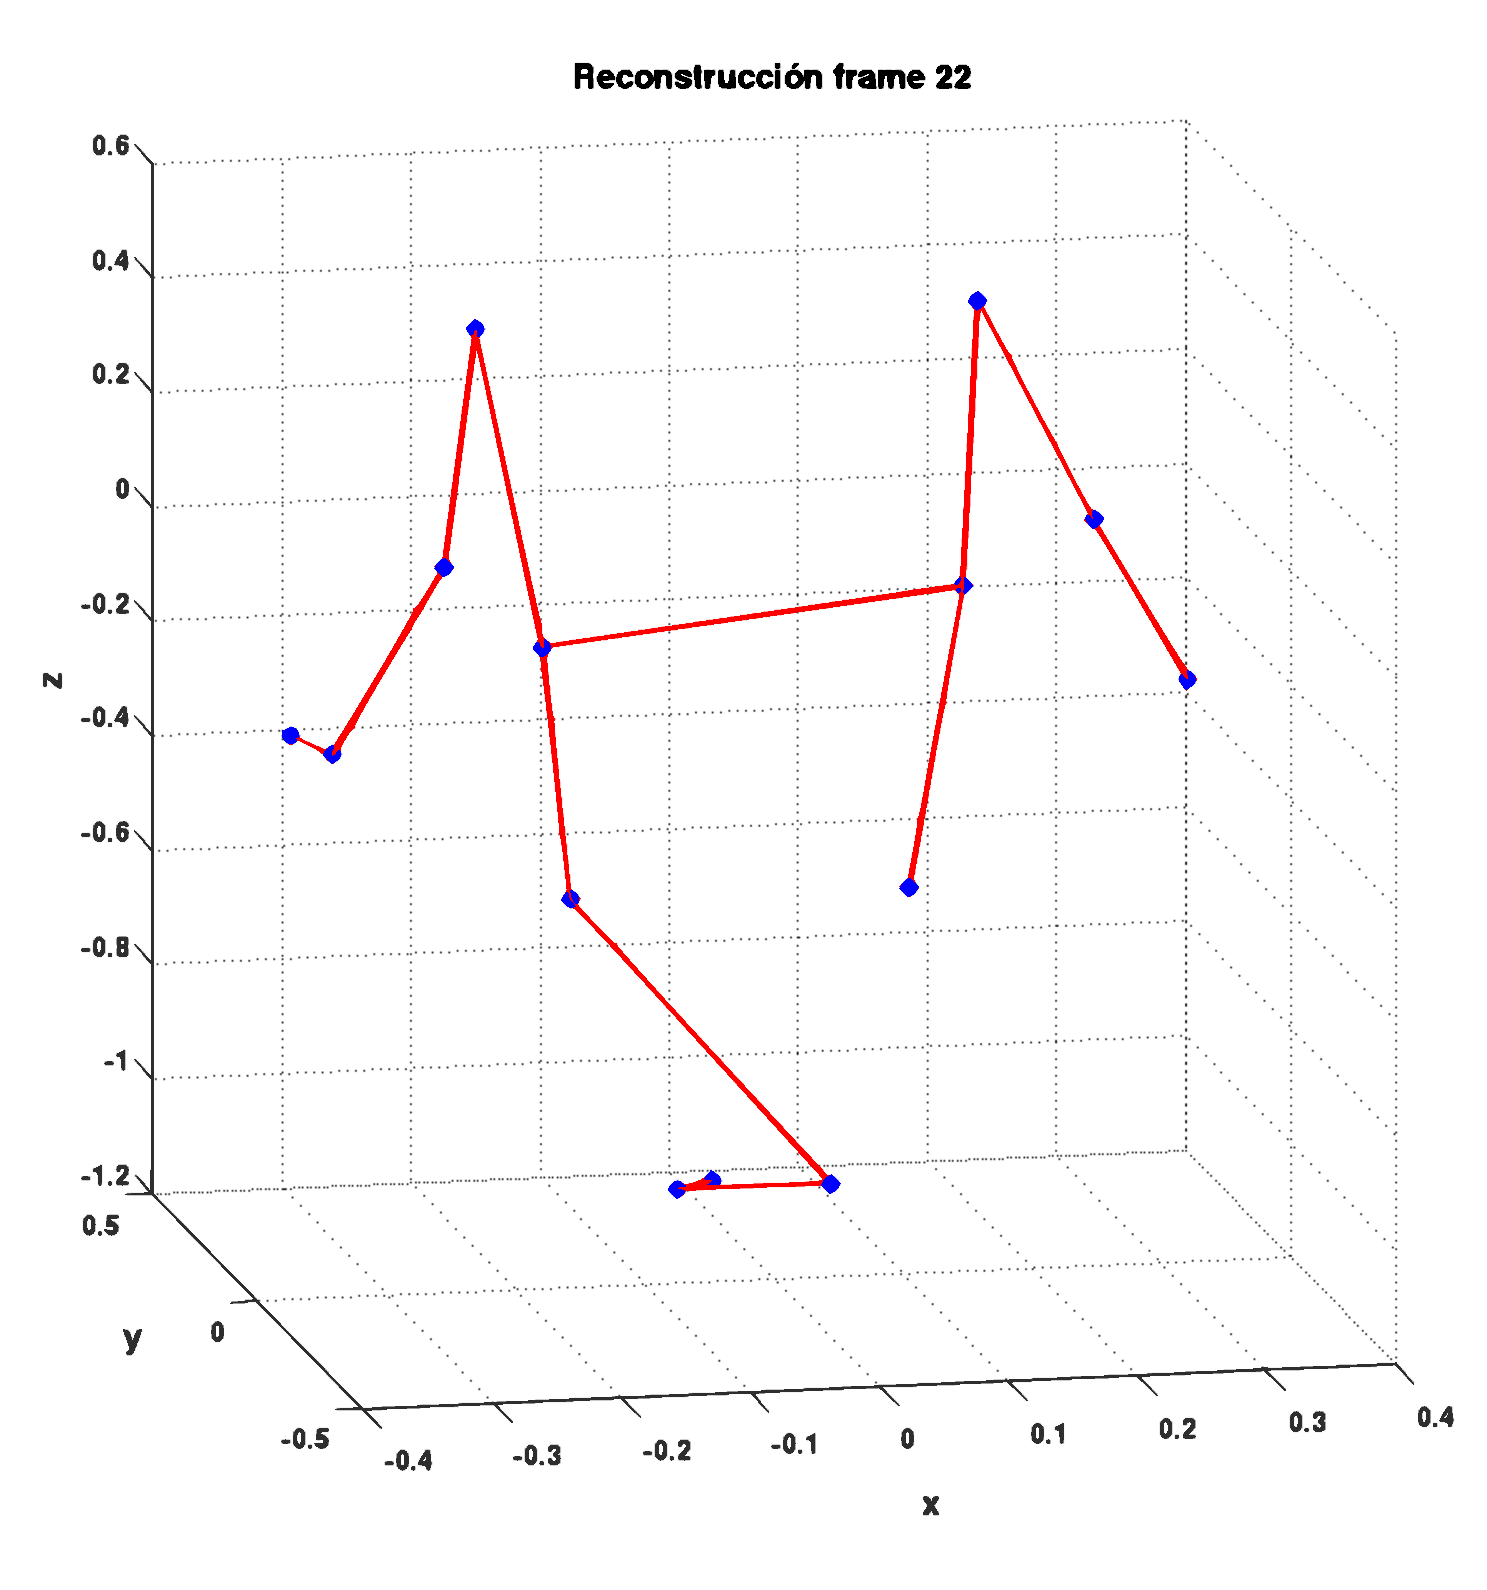
\includegraphics[scale=0.23]{img/Reconstruccion/frame22_esqueleto_armado.pdf}}
   \caption{Reconstrucción de una secuencia real.\\ Los asteriscos rojos indican los marcadores detectados.} 
   \label{img_reconstruccion_real2}    
\end{figure} 


\section{Conclusión} 

Tomando como punto de partida las ideas propuestas por Herda referentes a la reconstrucción de puntos 3D a partir de múltiples imágenes de puntos sobre distintas cámaras,  se han diseñado e implementado dos variantes de algoritmo principal para la etapa de reconstrucción. Logrando probar dichos algoritmos sobre secuencias tanto sintéticas como reales se hace un análisis cualitativo de los resultados.


Inicialmente se genera un algoritmo con etapas bien definidas (ver figura \ref{fig: diagrama algoritmo}), que obtiene resultados aceptables para secuencias sintéticas y configuraciones de más de 6 cámaras. Como es de esperar la configuración espacial de las cámaras influye en el desempeño del algoritmo por lo que valor anterior se obtiene asumiendo una distribución de cámaras uniforme alrededor del espacio de captura.


Las pruebas realizadas sobre secuencias reales dejan presente el problema de desempeño que tiene el algoritmo cuando se utilizan pocas cámaras, produciendo resultados poco satisfactorios. 
En nuestro caso las secuencias reales obtenidas manejan tan solo tres cámaras y las condiciones de laboratorio no son las favorables para efectuar un proceso de detección adecuado. Se ha visto que es necesario robustecer las etapas tanto de detección de marcadores  como de calibración, pues las incertidumbres producidas en dichas etapas tienen un efecto crítico sobre el desempeño de la reconstrucción. Con las secuencias reales disponibles, la falta de marcadores sobre las cámaras en la etapa de detección es la mayor dificultad a enfrentar al intentar reconstruir. 



Con el fin de independizarnos de los efectos de etapas anteriores, se introduce una secuencia sintética que simula el caso real, tanto en la calidad del movimiento como en el número y disposición de cámaras, donde los errores de calibración y detección de marcadores no son significativos.


Utilizando esta secuencia se implementa un nuevo algoritmo que mejora el desempeño en secuencias con pocas cámaras. Este nuevo algoritmo modifica parcialmente algunas etapas del algoritmo inicial, sobre todo la etapa de “Asociar puntos 2D”, logrando obtener resultados significativamente mejores al tratar con pocas cámaras sobre el caso sintético.
Utilizando las secuencias reales, se obtiene mejoras cualitativas sobre el primer algoritmo, si bien el desempeño es inferior al caso sintético y la reconstrucción es apenas aceptable.  \\ 


De lo expuesto se desprenden fundamentalmente dos cosas,
\begin{itemize}
\item las dificultades que ofrece el caso real fundamentalmente en la detección de marcadores y como esto influye significativamente en la etapa de reconstrucción perjudicando el resultado final del sistema.
\item el número de cámaras cambia significativamente el problema. Por un lado se genera un algoritmo que gestiona de manera aceptable la redundancia de información que existe cuando se utiliza un número de cámaras superior al necesario para cubrir un cierto espacio de captura. Dada las características de los movimientos tratados en este proyecto, básicamente de marcha rectilínea, nuestro límite inferior para  una reconstrucción aceptable son 6 cámaras.

 Por otro lado efectuando modificaciones al algoritmo anterior se genera un nuevo algoritmo, que permite trabajar con pocas cámaras pero no gestiona adecuadamente la redundancia de información.
\end{itemize} 

El análisis en biomecánica exige restricciones sobre precisión espacial en los resultados de la reconstrucción, por lo que resulta necesario optimizar esta etapa. 

De lo visto en la bibliografía existente podría proponerse el uso de la información de esqueleto, que impone restricciones sobre las posiciones de los marcadores. Si bien este tipo de análisis se menciona en el algoritmo propuesto por Herda, se decide en este trabajo generar un algoritmo en principio más generales y no se incorpora la información de esqueleto. \\
%VER CON GUILLERMO QUE QUISO PONER EN UNOS COMENTARIOS QUE ME PASO
 
 
 
%
%
%->Reconstrucción con base de datos sintética
%\\
%HABLAR Y MOSTRAR RESULTADOS DE La performance DE LA BASE DE DATOS AL UTILIZAR LAS DOS RAMIFICACIONES\\
%PROCEDIMIENTO DE ASOCIACIONES DEL TIPO TODO CONTRA TODO, Y ASOCIACIONES CON CÁMARAS CONSECUTIVAS.\\
%JUSTIFICAR POR LO TANTO QUE OFICIALMENTE NOS QUEDAMOS CON EL CASO DE ASOCIACIONES ENTRE CÁMARAS CONSECUTIVAS
%\\
%-----\\
%->CASO REAL
%\\
%\begin{itemize}
%\item introducción: SE PRUEBA SOBRE LO QUE SE TIENE DEL SISTEMA Y NO ANDA POR TAL Y TAL MOTIVO. pUES LA CALIBRACIÓN ES DIFERENTE NO SE OBTIENE RESULTADOS ACEPTABLES.
%
%\item EXPLICAR AJUSTE REALIZADOS, GENERACIÓN DE MINI-SISTEMA DONDE CORREN SECUENCIAS REALES.AQUÍ DEBE ESTAR EL NUEVO ALGORITMO DE RECONSTRUCCIÓN
%\begin{itemize}
%\item para todos los puntos contenidos en las retinas se trazan las correspondientes rectas de proyección 3D
%\item BLOQUE ASOCIACIÓN 3D: se asocian las rectas utilizando una métrica de distancia euclídea Las rectas de proyección que se encuentran a menor distancia entre si quedan asociadas.
%\item BLOQUE MEJOR ASOCIACIÓN: se elijen las n mejores asociaciones entre rectas 3D
%\item BLOQUE RECONSTRUCCIÓN: se reconstruyen los puntos 3D provenientes de las asociaciones anteriores 
%\end{itemize}
%
%\item EN DICHO MINI-SISTEMA SE SIMULA EN BLENDER EL CASO REAL Y SE INTENTA TENER ALGO MODERADAMENTE FUNCIONAL
%
%\item RESULTADOS -->ALGORITMO DE RECONSTRUCCIÓN OFICIAL(CASO ASOCIACIÓN ENTRE CÁMARAS CONSECUTIVAS) -->NO TUVO BUENOS RESULTADOS 
%\item CONSECUENCIA SE GENERA NUEVO ALGORITMO DE RECONSTRUCCIÓN QUE HACE TAL Y TAL COSA.
%\item CON ESTE NUEVO ALGORITMO SE OBTIENEN RESULTADOS ACEPTABLES SOBRE LAS SIMULACIONES DEL CASO REAL
%SE PRUEBA DICHO ALGORITMO SOBRE LOS DATOS REALES Y SE OBTIENEN RESULTADOS ACEPTABLES.
%\item JUSTIFICAR QUE LAS DIFERENCIAS SON DEBIDAS A CALIBRACIÓN (REAL VS SINTÉTICA) Y LA SEGMENTACIÓN (REAL VS SINTÉTICA).
%\item ¿CUALITATIVAMENTE SE PUEDE DECIR CUAL ES EL FACTOR QUE PERJUDICA EN MAYOR MEDIDA LOS RESULTADOS en la secuencia real RESPECTO AL CASO DE SIMULACIÓN SINTÉTICA?. Si la segmentación es lo que perjudica más, por tal y tal motivo.
%\end{itemize}
%
%\textbf{HABLAR DE LA INTEGRACIÓN DE ESTE NUEVO ALGORITMO EN EL SISTEMA COMPLETO.\\}
%\begin{itemize}
%\item para muchas cámaras (mas de 5 o 6, ver las pruebas de gonzalo) el sistema funciona razonablemente con la reconstrucción ``original''. Principalmente debido a que se cuenta con información redundante de los marcadores.
%\item para pocas cámaras se utiliza el nuevo algoritmo de reconstrucción, permite trabajar con la secuencia real disponible. con muchas cámaras el algoritmo puede ser computacionalmente complejo.
%\item explicar bien cual es la frontera entre uno y otro caso (5 o 6 cámaras?)
%\end{itemize}


